
%--------------------------------------------------------------------
%   Introduction
%--------------------------------------------------------------------

\section{Introduction}

With the discovery of the Standard Model (SM) Higgs boson at 
the CERN Large Hadron Collider (LHC) experiments and subsequent 
measurement of its parameters, the fundamental parameters of the 
SM have been measured directly and with remarkable precision.
To fully map out the validity of the theory of electroweak
interactions, further high-precision electroweak measurements 
have to be performed. Such high-precision measurements can also  
be considered as a portal to new physics, since non-SM contributions 
may lead to significant deviations for some precisely measurable 
and calculable observables. 

The Large Hadron-electron Collider
(LHeC)~\cite{AbelleiraFernandez:2012cc,Bruning:2019scy,%
Bruning:2706220} planned at the LHC may complement the proton ring 
with an electron beam, allowing to perform deep inelastic scattering 
(DIS) with electrons and protons up to TeV energies. Its kinematic 
reach to higher scales in comparison to HERA and the large expected 
integrated luminosity will allow for the first time to perform 
high-precision electroweak measurements at high scales in DIS.  

Since the discovery of weak neutral currents in 
1973~\cite{Hasert:1973ff,Haidt:2015bgg} and the formulation 
of the Glashow-Weinberg-Salam
model~\cite{Glashow:1961tr,Weinberg:1967tq,Weinberg:1971fb, 
Weinberg:1972tu,Salam:1964ry,Higgs:1964ia,Higgs:1964pj, 
Englert:1964et}, deep-inelastic lepton nucleon scattering has 
played an important role in testing the Standard Model. 
The first measurement of the weak mixing angle, $\sin^2 \theta_W$,  
was obtained from polarized electron deuteron scattering at SLAC 
\cite{Prescott:1978tm,Prescott:1979dh}. With the advent of HERA, 
the first electron proton collider, studies of the electroweak 
interactions could be extended to a much larger range of 
momentum transfer squared, $Q^2$. First measurements of
electroweak effects at HERA have been undertaken in 
Refs.~\cite{Ahmed:1994fa,Aktas:2005iv} and
more complete electroweak analyses have been performed only recently,
for example with the complete set of H1 data in Ref.~\cite{Spiesberger:2018vki}.
{\color{brown}
  For electroweak effects to become important, in particular the reach to higher values
  of \Qsq\ is of relevance.
  }

Apart from the LHeC, other options for experimentation with 
DIS are presently studied.
An electron-hadron collider is part of the
possible Future Circular Collider (FCC), the 
FCC-$eh$~\cite{Abada:2019lih}, and may reach even higher center-of-mass 
energies than the LHeC. At lower energies, the planned and 
approved Electron Ion Collider 
(EIC)~\cite{Accardi:2012qut,Aschenauer:2017jsk,EICpreCDR}
could extend DIS experiments towards higher luminosities and 
heavier nuclei.
For comparison, in Fig.~\ref{fig:dSigmaFacilities} we show  
single-differential neutral and charged current (NC and CC) 
inclusive DIS cross sections for polarized electron-proton 
scattering as a function of \Qsq\ comparing the future 
facilities LHeC, FCC-$eh$, and EIC, with H1 data from the past HERA
collider~\cite{Aaron:2012qi}.  
%
\begin{figure}[t!hb]
  \centering
  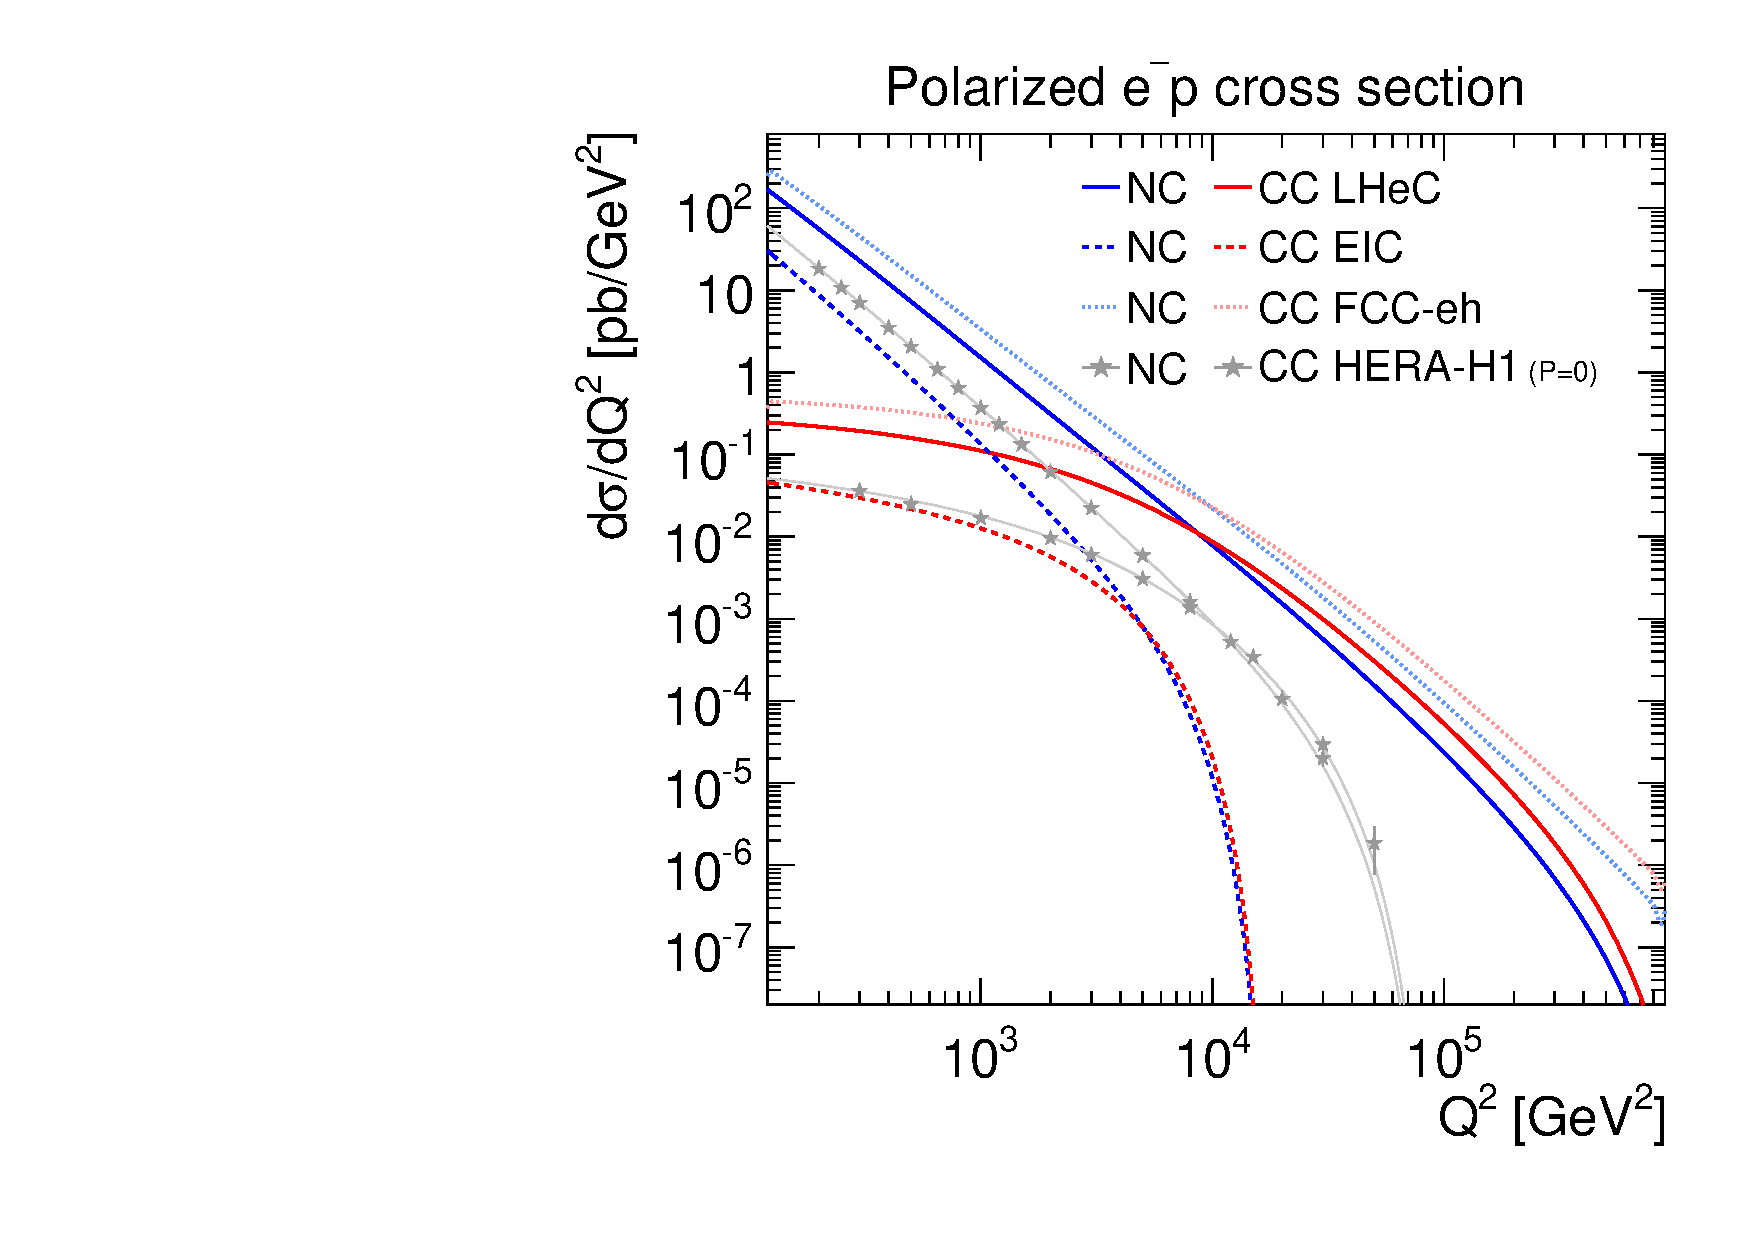
\includegraphics[width=0.56\textwidth]{plot_GraphsDsigmaDQ2_FCCEIC_opt}
  \caption{
    Single differential inclusive DIS cross sections for
    neutral and charged current $e^-p$ DIS with longitudinally polarized electrons ($P_e=-0.8$) at LHeC, 
    EIC, FCC-$eh$, and HERA.
    For HERA, unpolarized cross sections are displayed together with data from the H1 experiment.
  }
  \label{fig:dSigmaFacilities}
\end{figure}


The main physics motivation of the EIC lies in studies
of the strong interaction and the nucleon structure, and due to its
lower center-of-mass energy, it is not well suited for our purpose of
studies of electroweak physics\,\footnote{However, it is 
  expected, that also EIC may contribute to electroweak
  physics as well~\cite{Zhao:2016rfu}.
}.
The realisation of the FCC-$eh$ is in the far future and its configuration
and beam parameters are quite uncertain.
The LHeC, however, might be realized during the lifetime of the LHC and could 
start taking data in the 2030s. The LHeC has recently been 
described as a realistic option in the EPPSU deliberation 
document~\cite{European:2720131}. The newly proposed energy-recovery 
linac (ERL) for a high-quality electron beam, together with the 
high-luminosity upgrade of the LHC (HL-LHC), are expected to 
provide an extraordinary increase of the integrated luminosity, 
and consequently a significant increase in the reach towards 
higher \Qsq\ compared to what was assumed in all previous studies. 
This motivates us to perform this exploratory study for the LHeC 
and investigate the new possibilities for the measurement of 
electroweak physics effects. Studies of electroweak effects for 
similar energies have been performed in the past for the 
LHeC~\cite{AbelleiraFernandez:2012cc} and earlier, to some extent, for the 
LEP$\otimes$LHC proposal \cite{Jarlskog:1990bk}. 

We will put our focus on the measurement of inclusive NC and CC 
cross sections at the LHeC with the aim to determine parameters 
of the electroweak interaction. Measurements in the regime of 
spacelike momentum transfer, where the interaction is mediated 
by gauge boson exchange in the $t$-channel, is often complementary 
to other experiments, such as proton-proton collisions or 
electron-positron annihilation, or experiments at lower energies, 
like neutrino or muon scattering. The potential of experiments 
at the LHeC with exclusive final states, for example $W$- or 
$Z$-boson production, or production of the Higgs boson, has 
been studied elsewhere~\cite{Baur:1991pp,Baur:1989gh,Blumlein:1992eh,Li:2017kfk};
the possible improvement in our knowledge of parton distribution functions 
due to LHeC experiments was described in Refs.~\cite{Klein:1564929,AbdulKhalek:2019mps}
(see also Refs.~\cite{AbelleiraFernandez:2012cc,Abada:2019lih,Bruning:2706220} and references therein).

Our goal is to study tests of the electroweak SM. We therefore 
start with laying out the theoretical framework and summarize the 
SM predictions for NC and CC DIS cross sections, including 
higher-order electroweak corrections in the following section 
\ref{sec:theo}. In subsequent sections we describe the main 
features of the cross section predictions 
(Sec.\,\ref{sec:xsections}), the simulated data that we use 
(Sec.\,\ref{sec:data}), and the methodology for fitting these 
data to extract electroweak physics parameters  
(Sec.\,\ref{sec:fitmethods}). Then we present a first group of 
results in Sec.\,\ref{sec:mass} for the determination of mass 
parameters, i.e.\ the masses of the $W$ and $Z$ bosons and in 
Sec.\,\ref{sec:sw2eff} for the weak mixing angle. The expected high 
precision of measurements at the LHeC could allow us to also 
envisage an indirect determination of the top-quark mass through 
higher-order corrections (Sec.\,\ref{sec:mt}). These studies 
will allow one to perform tests of the SM by comparing 
different determinations of the electroweak physics parameters. 
Agreement with the theory can be quantified by the precision 
with which SM parameters are expected to be determined. 

In addition, we will study a number of possible ways to 
generically parametrize new physics beyond the SM and investigate 
the precision that can be obtained for limits on corresponding  
new parameters not present in the SM. In Sec.\,\ref{sec:stu} 
we study the well-known $STU$-parameters which describe new 
physics entering through loop insertions in the self energy 
corrections of the gauge bosons. Then we follow the wide-spread 
convention to generalize the SM gauge-boson fermion couplings 
by introducing $\rho$ and $\kappa$ parameters, both for NC 
(Sec.\,\ref{sec:rhokappa}) and for CC (Sec.\,\ref{sec:ewcc}), 
or, eventually, allowing the vector and axial-vector coupling 
constants to be independent free parameters, not obeying any 
restriction as imposed by the SM (Sec.\,\ref{sec:nccouplings}). 
We will be able to show that in particular the quark coupling 
constants, separately for up- and down-type quarks, can be 
determined with a precision at the sub-percent level. The 
large kinematic reach of the LHeC will also allow us to 
study the scale-, i.e.\ \Qsq-dependence of coupling parameters. 
This opportunity is in fact unique to the LHeC. 
Finally, we conclude and summarize the most important results 
in Sec.\,\ref{sec:conclusions}. The impact of the LHeC 
measurements on possible future global fits of the electroweak 
SM parameters is discussed in an appendix (\ref{app:globalfit}). 

% Some extra references: 
%
% muon life-time measurements~\cite{Tishchenko:2012ie}
%
% neutrino scattering experiments~\cite{Fogli:1988tv, 
% Blondel:1989ev,Allaby:1987vr,McFarland:1997wx,Zeller:2001hh},
%
% precision measurements at the $Z$ pole 
% and at even higher 
% scales~\cite{ALEPH:2005ab,Chatrchyan:2011ya,Schael:2013ita, 
% Aaij:2015lka,Aad:2015uau,Aaltonen:2018dxj}.


%--------------------------------------------------------------------
%   Theory
%--------------------------------------------------------------------
\clearpage

\section{Electroweak effects in inclusive NC and CC DIS}
\label{sec:theo}

In this section we lay out the general 
properties of DIS cross sections, first at leading order, 
taking into account single boson exchange diagrams at tree level. 

Inclusive NC DIS cross sections are expressed in terms of
generalised structure functions $\tilde{F}_2^\pm$, 
$x\tilde{F}_3^\pm$ and $\tilde{F}_{\rm L}^\pm$ at electroweak 
(EW) leading order (LO) as
\begin{equation}
\frac{d^2\sigma^{\rm NC}(e^\pm p)}{dxd\Qsq} 
= 
\frac{2\pi\alpha^2}{xQ^4} 
\left[Y_+\tilde{F}_2^\pm(x,\Qsq) 
     \mp Y_{-} x\tilde{F}_3^\pm(x,\Qsq) 
     - y^2 \tilde{F}_{\rm L}^\pm(x,\Qsq) 
\right]~,
\label{eq:cs}
\end{equation}
where $\alpha$ denotes the fine structure constant, $x$ is the
Bjorken scaling variable, and $y$ the inelasticity. The factors 
$Y_\pm = 1\pm(1-y)^2$ encode the helicity dependence of the 
underlying lepton quark hard-scattering process. The generalised 
structure functions can be separated into contributions from 
pure $\gamma$- and $Z$-exchange, and their 
interference~\cite{Klein:1983vs}:
\begin{eqnarray}
  \tilde{F}_2^\pm
  &=& F_2
  -(\ve\pm P_e\gae)\varkappa_ZF_2^{\gamma Z}
  +\left[(\ve\ve+\gae\gae)\pm2P_e\ve\gae\right]\varkappa_Z^2F_2^Z~,
\label{eq:strfun1}
  \\
  \tilde{F}_3^\pm
  &=& ~~~~
  -(\gae\pm P_e\ve)\varkappa_ZF_3^{\gamma Z}
  +\left[2\ve\gae\pm P_e(\ve\ve+\gae\gae)\right]\varkappa_Z^2F_3^Z~,
\label{eq:strfun2}
\end{eqnarray}
where $P_e$ is the degree of longitudinal polarization ($P_e = -1$ 
for a purely left-handed polarized electron beam). 
A similar decomposition exists for $\tilde{F}_L$.
%
The naive quark-parton model corresponds to the LO approximation 
of Quantum Chromodynamics (QCD). In this approximation the 
structure functions are calculated from quark and anti-quark 
parton distribution functions, $q(x)$ and 
$\bar{q}(x)$: 
\begin{eqnarray}
  \left[F_2,F_2^{\gamma Z},F_2^Z\right]
  &=& 
  x\sum_q\left[Q_q^2,2Q_q\vq,\vq\vq+\aq\aq \right]\{q+\bar{q}\}~
\label{eq:last1}
  \\
  x\left[F_3^{\gamma Z},F_3^Z\right]
  &=& 
  x\sum_q\left[2Q_q\aq,2\vq\aq\right]\{q-\bar{q}\}~. 
\label{eq:last2}
\end{eqnarray}
In Eqs.~\eqref{eq:strfun1} and~\eqref{eq:strfun2}, the 
coefficient $\varkappa_Z$ accounts for the $Z$-boson 
propagator and the normalisation of the weak, relative to the 
electromagnetic, interaction. It is calculated, at LO, as 
\begin{equation}
  \varkappa_Z(\Qsq)
  = \frac{\Qsq}{\Qsq+m^2_Z}
  \frac{1}{4\sw \cos^2\theta_W}
  = \frac{\Qsq}{\Qsq+m^2_Z}
  \frac{\gf m_Z^2}{2\sqrt{2}\pi\alpha}~. 
\label{eq:kappaZ-LO}
\end{equation}
Thus, depending on the choice of independent theory parameters, 
the normalization of $\varkappa_Z$ is fixed by an input value 
for $\sw$, or, alternatively, using the Fermi coupling constant 
$\gf$. The first option where $\sw = 1 - \cos^2\theta_W = 
1 - m_W^2/m_Z^2$ is fixed, is called the {\em on-shell scheme}, 
while the second option with $\gf$ as input parameter is known 
as the {\em modified on-shell scheme}. 

The vector and axial-vector coupling constants of the lepton 
or quark to the $Z$-boson, $g_V^{e/q}$ and $g_A^{e/q}$ in 
Eqs.~\eqref{eq:strfun1} and~\eqref{eq:strfun2}, are given by 
the SM electroweak theory. They depend on the electric charge, 
$Q_{q/e}$, in units of the positron charge, and on the third 
component of the weak-isospin of the fermion, $I^3_{{\rm L},q/e}$. 
They are given, at LO, by\,\footnote{In the following, we will use the subscripts $q$, $\ell$ and $f$ to refer generically to specific quark or lepton flavors or both, respectively, but also to universal, i.e.\ flavor indpendent, quantities. The meaning becomes clear from the context.}
\begin{eqnarray}
  g_A^{f} 
  &=& I^3_{{\rm L},f}
\label{eq:gA-LO} \,, \\
  g_V^{f} 
  &=& I^3_{{\rm L},f} - 2 Q_{f} \sw \, . 
\label{eq:gV-LO} 
\end{eqnarray} 

The CC DIS cross section is written, in the LO approximation, 
as 
\begin{equation}
  \frac{d^2\sigma^{\rm CC}(e^\pm p)}{dxd\Qsq}
  = \frac{1 \pm P_e}{2}
  \frac{\pi \alpha^2}{4\sin^4\theta_w} 
  \frac{1}{x}
  \left[\frac{1}{\Qsq+m_W^2}\right]^2
  \left(Y_+ W_2^\pm(x,\Qsq) \mp Y_{-} xW_3^\pm(x,\Qsq)
  - y^2 W_{\rm L}^\pm(x,\Qsq)\right)~.
\label{eq:cc-cs}
\end{equation}
Here, an incoming electron can scatter only with positively 
charged quarks. Therefore, in the naive quark-parton model the 
structure functions $W_2^\pm$ and $xW_3^\pm$ are obtained 
from parton distribution functions for up-type quarks and 
down-type anti-quarks as 
\begin{equation}
  W_2^- =
  x \left( U + \overline{D} \right)
  \, ,
  \quad xW_3^- =
  x \left( U - \overline{D} \right)
  \, ,
\label{eq:w23el-LO}
\end{equation}
where $U = u+c$ and $\overline{D} = \bar{d} + \bar{s}$. For 
positron scattering, the combinations $\overline{U} = \bar{u} 
+ \bar{c}$ and $D = d+s$ are needed and one has 
\begin{equation}
  W_2^+ =
  x \left( \overline{U} + D \right)
  \, , 
  \quad xW_3^+ =
  x \left( D - \overline{U} \right)
  \, . 
\label{eq:w23po-LO}
\end{equation}
At LO of QCD, one has for the longitudinal structure function 
$W_{\rm L}^\pm = 0$. 

Higher-order perturbative corrections of QCD are included in 
the $\overline{\rm MS}$ scheme by using $Q^2$-dependent parton 
distribution functions, $q(x, Q^2)$ and $\bar{q}(x, Q^2)$, 
evolved according to the 
Dokshitzer-Gribov-Lipatov-Altarelli-Parisi equations. 
In addition, there are corrections of order $O(\alpha_s)$ to 
the relations (\ref{eq:last1}, \ref{eq:last2}) and 
(\ref{eq:w23el-LO}, \ref{eq:w23po-LO}) between PDFs and 
structure functions, and the longitudinal structure functions 
for NC and CC are predictions of perturbative QCD. 

We will see below that the precision of LHeC measurements 
is expected to be at a level which makes the inclusion of 
higher-order electroweak corrections indispensable. One-loop 
EW corrections have been calculated in 
Refs.~\cite{Bohm:1986na,Bardin:1988by,Hollik:1992bz}
for NC and in Refs.~\cite{Bohm:1987cg,Bardin:1989vz} for CC
scattering (see also ref.~\cite{Heinemann:1998kk} for a study 
of numerical results). We have adapted the implementation in 
the program EPRC~\cite{Spiesberger:1995pr} for our present 
study. 

The dominating universal higher-order EW corrections can be 
described by a modification of the fermion gauge-boson couplings. 
For NC scattering, they are taken into account by replacing 
Eqs.~(\ref{eq:gA-LO}, \ref{eq:gV-LO}) with corrected couplings 
\begin{eqnarray}
  g_A^{f} 
  &=& \sqrt{\rho_{\text{NC}, f}} \, I^3_{{\rm L},f}
\label{eq:gA-NLO} \,, \\
  g_V^{f} 
  &=& \sqrt{\rho_{\text{NC}, f}} \, \left(I^3_{{\rm L},f} - 2
  Q_{f} \, \kappa_{f} \, \sw \right)
\label{eq:gV-NLO} \,.
\end{eqnarray} 
At LO, the coefficients $\rho_{\text{NC}, f}$ and 
$\kappa_{f}$ are unity, but at NLO they are promoted 
to form factors which are flavor and scale dependent. Since they 
depend on \Qsq, they render the coupling constants `effective' 
running couplings. The coefficient $\kappa_{f}$ can 
be combined with \sw\ to define an effective, flavor and scale-dependent ($\mu^2$)
weak mixing angle, 
\begin{equation}
  \sin^2 \theta_{W,f}^{\rm eff} (\mu^2) = 
  \kappa_{f}(\mu^2) \sw \, . 
\label{eq:sin2w-eff}
\end{equation} 
The leptonic weak mixing angle, $\sin^2 \theta_{W,\ell }^{\rm eff} 
(m_Z^2)$, has been used to describe LEP/SLD observables at the 
$Z$-pole (see e.g.~\cite{PDG2020}). We emphasize that the $\mu^2$ 
dependence of the effective weak mixing angle is not negligible 
for LHeC physics ($\mu^2 = - Q^2$), while only its value at 
$\mu^2 = +m_Z^2$ was relevant for $Z$-pole observables. 

For CC scattering, a corresponding correction factor 
$\rho_{\text{CC}, eq}$ is introduced for $e^- q$ and 
$e^+ \bar{q}$ scattering, and $\rho_{\text{CC}, e\bar{q}}$ 
for $e^- \bar{q}$ and $e^+ q$ scattering, by the replacement 
of Eqs.~(\ref{eq:w23el-LO}, \ref{eq:w23po-LO}) with 
\begin{equation}
  W_2^- =
  x \left( \rho_{\text{CC}, eq}^2 U 
  + \rho_{\text{CC},e\bar{q}}^2 \overline{D} \right)
  \, ,
  \quad xW_3^- =
  x \left( \rho_{\text{CC}, eq}^2 U 
  - \rho_{\text{CC},e\bar{q}}^2 \overline{D} \right)
  \, ,
\label{eq:w23el-NLO}
\end{equation}
and 
\begin{equation}
  W_2^+ =
  x \left( \rho_{\text{CC},e\bar{q}}^2 \overline{U} 
  + \rho_{\text{CC}, eq}^2 D \right)
  \, , 
  \quad xW_3^+ =
  x \left( \rho_{\text{CC},e\bar{q}}^2 D 
  - \overline{U} \rho_{\text{CC}, eq}^2 \right)
  \, . 
\label{eq:w23po-NLO}
\end{equation}
In addition, box graph corrections, which are $Q^2$- and 
energy-dependent, are added as separate correction terms to the 
NC and CC cross sections. Higher-order EW corrections are defined 
in the on-shell scheme~\cite{Sirlin:1980nh,Sirlin:1983ys}, 
using \mz\ and \mw\ as independent parameters (see also 
Refs.~\cite{Bohm:1986rj,Hollik:1988ii}).

In order to calculate predictions in the SM electroweak theory 
at LO, only two independent parameters are needed in addition 
to $\alpha$. At higher orders, loop corrections involve a 
non-negligible dependence on the complete set of SM parameters, 
where the most important ones are the top-quark mass, $m_t$, 
and the Higgs-boson mass, $m_H$. In addition, hadronic 
contributions to the running of the effective couplings 
have to be provided as independent 
input~\cite{Jegerlehner:1985gq,Jegerlehner:2011mw}, since the 
corresponding higher-order corrections can not be calculated 
in perturbation theory. 

In the on-shell scheme, the masses of all particles are 
taken as independent input parameters. The weak mixing angle 
is defined by the masses of the $W$ and $Z$ bosons, 
$\sw = 1-m_W^2/m_Z^2$, also at NLO. Since the Fermi constant 
\gf\ has been measured with a very high precision
in muon-decay experiments~\cite{Tishchenko:2012ie} it is 
often preferred to calculate the less well-known $W$-boson 
mass from the relation 
\begin{equation}
  \gf = \frac{\pi \alpha}{\sqrt{2} m_W^2} \frac{1}{\sw} 
  \frac{1}{1 - \Delta r} \, , 
\label{eq:deltar-NLO}
\end{equation}
where higher-order corrections enter through the
quantity $\dr =$ $\dr(\alpha,$ $m_W$, $m_Z$, $m_t$, $m_H, \ldots)$
\cite{Sirlin:1980nh}, which depends on all mass parameters 
of the EW SM. The correction \dr\ has also to be taken into 
account when the propagator factor $\varkappa_Z(\Qsq)$ (see 
Eq.~(\ref{eq:kappaZ-LO})) is calculated, using either 
$\alpha$, $m_W$ and $m_Z$ (the naive on-shell scheme), or 
$\alpha$, \gf\ and $m_Z$ (the modified on-shell scheme) to 
fix input parameters. The choice of a scheme for input 
parameters is important since it leads to very different 
sensitivities to parameter variations. 


%--------------------------------------------------------------------
%
%--------------------------------------------------------------------
\clearpage

\section{Inclusive DIS cross sections at the LHeC}
\label{sec:xsections}

The contribution of the weak interaction to inclusive NC and CC
DIS cross sections becomes large at large momentum transfers 
and competes with the purely electromagnetic interaction. This 
is most clearly illustrated in Fig.~\ref{fig:dSigma} where we 
show predictions for the single-differential cross sections for 
polarised $e^-p$ scattering as a function of \Qsq. Here, LHeC 
electron beam energies of $E_e=50~\GeV$ and 60~\GeV, and a 
proton beam energy of $E_p=7000~\GeV$ are chosen. The LHeC 
predictions are compared to data for unpolarized scattering 
measured at HERA, where the electron and proton beam energies 
had been $E_e = 27.6$~GeV and $E_p = 920$~GeV, respectively.  

\begin{figure}[b!]
  \centering
  \includegraphics[width=0.52\textwidth]{plot_GraphsDsigmaDQ2_LHeC}
  \caption{
      Single differential inclusive DIS cross sections for
      polarised $e^-p$ NC and CC DIS at the LHeC for two different 
      electron beam energies ($E_e=50$ and 60\,\GeV). Cross 
      sections for longitudinal electron beam polarisations of 
      $P_e=-0.8$ and $+0.8$ are displayed. For comparison also 
      data measured by H1 at HERA~\cite{Aaron:2012qi}
      at center-of-mass energies of $\sqrt{s}=920\,\GeV$ with 
      unpolarised ($P=0$) electron beams are displayed. 
      }
\label{fig:dSigma}
\end{figure}

At lower values of \Qsq, the NC cross section is dominated by
the photon-exchange contribution, determined by the structure 
function $F_2$ (c.f.\ Eqs.~(\ref{eq:strfun1}, \ref{eq:strfun2})), 
and much larger than the cross section for CC scattering. 
At values of \Qsq below the mass of the $W$ 
boson, $\Qsq\ll\mW^2$, the propagator term in the CC cross 
section becomes $\mW^2 / (\mW^2+\Qsq) \simeq 1$ and, 
therefore, the CC cross section depends only little on \Qsq.

Weak contributions to the NC cross section become important 
at \Qsq\ values around the electroweak scale, $\Qsq\approx\mZ^2$. 
As a consequence, the dependence of the NC cross section on 
the longitudinal beam polarisation, $P_e$, becomes strong, and 
the cross sections for positive and negative helicities differ 
significantly. Since CC scattering is purely left-handed, the 
dependence on the longitudinal beam polarisation is strongest 
in this case: the CC cross section scales linearly with the 
fraction of left-handed electrons in the beam, i.e.\ with 
$1 - P_e$ (c.f.\, Eq.~\eqref{eq:cc-cs}). Note that, since DIS 
is mediated by gauge boson exchange with spacelike momentum 
transfer, no resonance of a weak boson is present in the 
\Qsq-dependent cross section. 

The cross sections increase slowly with the center-of-mass 
energy, mainly because the reach towards smaller values of 
the Bjorken variable $x$ gets larger. For an electron beam 
energy of $E_e=60~\GeV$, the cross sections for NC or CC 
scattering in the typical range of \Qsq in $10\,000 < \Qsq 
< 100\,000~\GeVsq$ are larger by about 10 to 15~\%, compared 
with the case of $E_e=50~\GeV$. The difference of cross sections 
between $E_e=50$ and 60\,\GeV increases with \Qsq. 


%--------------------------------------------------------------------
%
%--------------------------------------------------------------------
\clearpage

\section{LHeC pseudo data}
\label{sec:data}

In this section, the details of the LHeC pseudo data\,\footnote{In 
   the following, the simulated \emph{pseudo data} is simply 
   denoted as \emph{data} in order to facilitate reading.}
used below for an extraction of electroweak parameters are 
described.

In the present analysis simulated double-differential inclusive NC and
CC DIS cross section data are exploited.
The data have been simulated based on a numerical
procedure~\cite{Blumlein:1990dj} for the purpose of the LHeC CDR
update~\cite{Bruning:2706220} and are available from
Ref.~\cite{MaxHome17,MaxHome19}.
The data are briefly described in the following.

The data sets include electron and positron scattering, 
different lepton beam polarisation settings, and different 
proton beam energies. Since a decision about the actual layout 
of the LHeC energy-recovery linac for the lepton beam has not 
yet been taken, we will study scenarios for two lepton beam
energies, i.e.\ $E_e = 50~\GeV$ and 60~\GeV. Most of the 
data were generated with the nominal LHC proton beam energy 
of $E_p = 7000~\GeV$, but in addition, a small sample with the 
reduced proton energy of $E_p = 1000$~GeV is also considered.
A summary of the data sets is given in Table~\ref{tab:datasets}.

\begin{table}[tbh!]
  \centering
  \small
  \begin{tabular}{lccccccc}
    \toprule
    Processes & $E_p$ & $Q_e$ & $P_e$ &
    $\mathcal{L}$ & \Qsq\ range & 
    \multicolumn{2}{c}{No. of data points (NC, CC)} \\
    \cmidrule(lr){7-8}
    &  [TeV] & & &  [fb$^{-1}$]&  [GeV$^2$] & LHeC-60 & LHeC-50  \\
    \midrule
    NC, CC &  7  & $-1$ &  $-0.8$ & 1000 & 5 -- $10^6$ 
       & 150, 114 & 150, 123
    \\ % D4
    NC, CC &  7  & $-1$ &  $+0.8$ & 10   & 5 -- $10^6$  
       & 150, 113 & 146, 117
    \\ % D8
    NC, CC &  7  & $+1$ &  $ 0  $ & 10   & 5 -- $5\cdot10^5$  
       & 148, 109 & 145, 111
    \\ % D7
    NC, CC &  1  & $-1$ &  $ 0  $ & 1    & 5 -- $10^5$  
       & 128, ~~93 & 120, ~~92
    \\ % D5
    \bottomrule
  \end{tabular}
  \caption{
    Summary of data sets used in our analysis. Each set is 
    simulated for the two electron beam energies $E_e=50~\GeV$ 
    and 60~\GeV. 
  }
  \label{tab:datasets}
\end{table}

The majority of the data will be collected with an electron
beam ($Q_e=-1$) and with a longitudinal beam polarisation
of $P_e=-0.8$, reaching an integrated luminosity of about
$\mathcal{L}\simeq1000~\textrm{fb}^{-1}$. This will allow 
us to consider measurements of NC and CC DIS cross sections 
up to values 
of $\Qsq\simeq1\,000\,000\,\GeVsq$. A considerably smaller 
data sample will be collected with a positive electron beam 
polarisation of $P_e=+0.8$, i.e.\ with right-handed electrons. 
For this sample, an integrated luminosity of 10\,fb$^{-1}$ 
was assumed. Another data sample will be collected with a 
positron beam, where it is assumed that polarisation will not 
be available. Technical limitations for the positron source 
put constraints on the achievable beam current and thus on 
the instantaneous luminosity. Therefore, an integrated luminosity 
of (only) 10\,fb$^{-1}$ is assumed for this sample.
Nonetheless, this will allow us to consider measurements with 
positrons up to \Qsq\ values of 500\,000\,\GeVsq. Finally, 
another data sample will be collected with a reduced proton beam
energy. This will be important for a determination of $F_L$ 
and to access higher values of $x$. For this low-energy sample 
an integrated luminosity of 1\,fb$^{-1}$ was assumed.
All data sets were restricted to $\Qsq\geq5\,\GeVsq$ in order 
to avoid regions where higher-order QCD effects are important, 
which could deteriorate the determinations of parton distribution 
functions. For our purpose, the low-\Qsq region is anyway of 
less interest since it does not contribute much to the 
sensitivity to EW parameters. CC DIS data are simulated only for 
$\Qsq\geq100\,\GeVsq$, since CC scattering events with lower \Qsq 
may be difficult to measure due to limitations of the trigger 
system.

The data simulation accounts for the acceptance of the LHeC
detector, the kinematic reconstruction, and trigger restrictions. 
The resulting coverage of the kinematic plane can be found, for
instance, in Ref.~\cite{AbdulKhalek:2019mps}. 

\begin{table}[tbh!]
  \centering
  \small
  \begin{tabular}{lccc}
    \toprule
    Source of uncertainty & Size of uncertainty & \multicolumn{2}{c}{Uncertainty on cross section} \\
    \cmidrule(lr){3-4}
    &  & $\Delta\sigma_\textrm{NC}$ & $\Delta\sigma_\textrm{CC}$ \\
    \midrule
    Scattered electron energy scale $\Delta E_e' /E_e'$ & 0.1 \%  & 0.1 -- 1.7\,\% &   \\
    Scattered electron polar angle  & 0.1\,mrad  &   0.1 -- 0.7\,\% &    \\
    Hadronic energy scale $\Delta E_h /E_h$ & 0.5\,\%  & 0.1 -- 4\,\% &  1.0 -- 8.6\,\%  \\
    Calorimeter noise (only $y < 0.01$) & 1\,--\,3\,\%  & 0.0 -- 1.1\,\% &    \\
    \addlinespace    
    Radiative corrections &  &  0.3\,\%  &  \\
    Photoproduction background ($y > 0.5$) & 1\,\%  & 0.0 or 1.0\,\% &    \\
    %Global efficiency uncertainty &   &  0.5\,\%  &   0.5\,\%   \\ that's the uncorrel. uncertainty
    Uncorrelated uncertainty (efficiency) &  &  0.5\,\% &   0.5\,\%  \\ % Global efficiency error
    Luminosity uncertainty (normalisation) & & 1.0\,\%   &  1.0\,\%    \\
    \bottomrule
 \end{tabular}
\caption{
  Summary of the assumptions for uncertainties from various 
  sources used in the simulation of the NC cross sections.
  The first three items are calibration uncertainties and 
  affect the event reconstruction. The last four items are 
  uncertainties which can be assigned directly to the cross 
  section. 
}
\label{tab:uncert}
\end{table}

The data include a full set of systematic uncertainties and
the individual sources are summarised in Table~\ref{tab:uncert}. 
For the bulk of the phase space, the `electron' 
reconstruction method is used where the kinematic variables $x$ and 
$Q^2$ are determined from the energy and polar angle of the 
scattered electron. Important uncertainties originate from the 
electron energy scale and polar angle measurement, and
uncertainties of $\Delta E_e^\prime / E_e^\prime = 0.1~\%$ and
$\Delta\theta^\prime_e = 0.1$~mrad are assumed. However, at lower values of 
$y$ the so-called `mixed' reconstruction
method~\cite{Blumlein:1990dj} has to be employed which makes 
use of the measurement of the hadronic final state to 
determine $y$ and $x=\Qsq/(sy)$. %$y_h=\tfrac{\Sigma}{2E_e}$.
For the measurement of the hadronic final state, an uncertainty 
on the hadronic energy scale of $\Delta E_h/E_h = 0.5~\%$
is imposed. Furthermore, uncertainties from QED radiative 
corrections of 0.3~\%, and an uncertainty due to the background 
from photoproduction events of $1.0~\%$ in the high-$y$ region 
is assumed. The statistical uncertainty is taken to be at least 
0.1~\%. A global normalisation uncertainty of 1~\% is taken into 
account, which includes the luminosity uncertainty. Finally, 
a potential additional source of measurement errors is combined 
in an uncorrelated uncertainty component of 0.5\,\%.
These may comprise unfolding and model uncertainties, efficiency
uncertainties, beam background related uncertaintes, or further
uncertainties related to the calibration procedure.

The data samples that we use have originally been simulated 
mainly for the purpose to perform studies of PDF determinations.  
These are sensitive to the lower-\Qsq region, while the present 
study of electroweak parameter determinations is dominated 
by high-\Qsq data. For simplicity, a coarse $x$-\Qsq
grid for the simulated data points was chosen (see 
Table~\ref{tab:datasets}), but real data may allow a much finer 
binning, in particular at medium $x$ values or at higher \Qsq. 
A finer binning can be simulated to a very good approximation 
by changing the size of the uncorrelated uncertainty. 
In the following, we will consider two alternative scenarios, 
one based on the original binning and with an uncorrelated 
uncertainty of 0.5~\%, as well as a more optimistic setting 
where the grid in both $x$ and \Qsq is assumed finer by a 
factor of 2 and emulated by choosing the uncorrelated uncertainty 
correspondingly improved by the same factor, i.e.\ equal to 
$0.25\,\%$. The statistical uncertainty is determined by the 
expected number of events; however, we keep in any case a 
minimum value of 0.1~\% for every data point. The properties 
of the four sets of data samples which we will use are collected 
in Table\,\ref{tab:scenarios}.

\begin{table}[thb!]
  \centering
  \small
  \begin{tabular}{lccc}
    \toprule
    Scenario & $E_e$ & No. of data points (bin grid)\\
    \midrule
    LHeC-50a  &   50\,\GeV&  nominal            \\
    LHeC-50b  &   50\,\GeV&  4$\times$ nominal  \\
    LHeC-60a  &   60\,\GeV&  nominal            \\
    LHeC-60b  &   60\,\GeV&  4$\times$ nominal  \\
    \bottomrule
 \end{tabular}
  \caption{
    Summary of the LHeC measurement scenarios. They will be 
    referred to by the names shown in the first column. For 
    the 'a'-scenarios, the uncorrelated uncertainty is chosen 
    equal to 0.5~\%. In the last column we indicate that a 
    reduced uncorrelated uncertainty of 0.25~\% for the 
    'b'-scenarios can be realized by increasing the number of 
    bins with respect to the \emph{nominal} number of data 
    points (see table~\ref{tab:datasets}). 
  }
  \label{tab:scenarios}
\end{table}

We should point out that the large number of data points, in the 
order of a few hundred, allows us to consider the data essentially 
as a collection of cross section ratios. In previous studies (see, 
e.g.~\cite{Blumlein:1987fd,Spiesberger:1993jg}) it was often 
assumed that such ratios are measured directly, for example the 
ratio of CC over NC cross sections, $R_{\rm CC/NC}$, the 
polarization asymmetry $A_{\rm LR}$ or the charge asymmetry 
$B_{\pm}$ measuring the difference between cross sections 
for electron and positron scattering. We do not construct 
these ratios explicitly, but leave it to the parameter
extraction procedure to exploit implicitly
the corresponding information. We can then expect that 
most of the correlated uncertainties, e.g.\ normalization
uncertainties, become largely constraint by the fit
while uncorrelated uncertainties are reduced by taking 
the properly weighted average of all data. As a consequence, 
uncertainties at the per mille level can be expected for the 
observables which we are going to study in the sequel. The 
two measurement scenarios labeled with `a' and `b' described 
above will help us to verify this rough estimate of exptected 
parameter uncertainties and its dependence on our assumption 
for correlated measurement errors. 


%--------------------------------------------------------------------
%   Methodology
%--------------------------------------------------------------------
\clearpage

\section{Methodology of a combined EW+PDF fit}
\label{sec:fitmethods}

By the time when the LHeC is realized, one should expect that 
the determination of PDFs will be dominated by NC and CC DIS 
data obtained there. The uncertainties of PDF parametrizations 
will mainly represent the propagated uncertainties of these 
inclusive LHeC data. The uncertainties of EW parameters determined 
from cross section data will therefore be correlated with PDF 
uncertainties. In order to account for these correlations, EW 
parameters have to be determined in a combined fit simultaneously 
with PDFs. This allows us to take into account the complete 
set of statistical, as well as correlated and uncorrelated 
systematic uncertainties. We denote such an approach in the 
following by `EW'+PDF fit, while `EW' may be replaced by the parameter
of interest.

The $x$-dependence of the PDFs is parametrised at a starting 
scale of $\mu_0 = 1.3784~\GeV$, i.e.\ below the charm threshold.
Five PDFs are chosen as independent input at this scale: 
the $u$ and $d$ valence quark distributions ($xu$ and $xd$), 
the $u$-type and $d$-type anti-quark distributions ($x\overline{U}$ 
and $x\overline{D}$), and the gluon distribution ($xg$). The choice 
of the parametrisation follows previous LHeC PDF
studies~\cite{AbelleiraFernandez:2012cc,Klein:1564929}, 
which are closely related to HERAPDF-style
PDFs~\cite{Adloff:2000qk,Abramowicz:2015mha,Andreev:2017vxu}. 
The following functional form is used: 
\begin{equation}
  xf = f_A x^{f_B} (1-x)^{f_C} (1+f_Dx+f_Ex^2) -
      f_{A^\prime}x^{f_{B^\prime}}(1-x)^{0.25}\,,
\end{equation}
where $f$ denotes any of the five input PDFs, $f = u$, $d$, 
$\overline{U}$, $\overline{D}$, $g$. The second term in this ansatz is 
taken into account only for the gluon distribution\footnote{
   The second term is commonly considered 
   to be of importance for PDF determinations as it introduces 
   additional freedom at lower values of $x$. This may be 
   important to describe LHeC data which probes the $x$ region 
   down to $x \simeq 5\cdot10^{-6}$. However, we find that 
   this has no significant impact on the resulting uncertainties 
   of the electroweak parameters.}, i.e.\ 
$u_{A^\prime} = d_{A^\prime} = \overline{U}_{A^\prime} = 
\overline{D}_{A^\prime} = 0$. The normalisation of each PDF is 
determined by the quark number sum-rule ($u_A$, $d_A$) or 
the momentum sum-rules ($g_A$). For the anti-quark PDF, we fix 
$\overline{U}_A = \overline{D}_A(1-0.4)$. Furthermore, we use $\overline{D}_B = 
\overline{U}_B$. Altogether, 13 independent PDF parameters are 
determined in each fit ($g_B$, $g_C$, $g_{A^\prime}$, 
$g_{B^\prime}$, $u_B$, $u_C$, $u_E$, $d_B$, $d_C$, $\overline{U}_C$, 
$\overline{D}_A$, $\overline{D}_B$, $\overline{D}_C$). The values of the PDF 
parameters used for the generation of pseudo data are not of 
particular relevance here. They have been obtained from a 
private fit to HERA data, similar to Refs.~\cite{Aaron:2012qi,Andreev:2017vxu}. 

QCD higher-order corrections are taken into account at NNLO 
in the zero-mass variable flavor number scheme. They are 
implemented for the evolution of the PDFs and the calculation 
of the structure functions using 
QCDNUM~\cite{Botje:2010ay,Botje:2016wbq}.  
We do not consider QED or EW corrections for the PDF 
evolution~\cite{DeRujula:1979grv,Kripfganz:1988bd,
Blumlein:1989gk,Spiesberger:1994dm}, since their impact on 
the determination of EW parameters is expected to be small 
and does not change the uncertainties estimated in the present 
study. EW effects are, however, included in the calculation 
of cross sections, as described above in Sec.~\ref{sec:theo}. 

The $\chi^2$ quantity which is subject to the minimisation and
error propagation is based on normal-distributed relative
uncertainties,
\begin{equation}
  \chi^2 =\sum_{ij} \log{\frac{\varsigma_i}{\sigma_i}}V^{-1}_{ij}
  \log{\frac{\varsigma_j}{\sigma_j}}
\end{equation}
where the sum runs over all data points, $\varsigma_i$ are the 
measured cross section values and $\sigma_i$ their corresponding 
theory predictions (c.f.\ Eqs.~\eqref{eq:cs} and~\eqref{eq:cc-cs}),
which incorporate the dependence on the fit parameters. The covariance 
matrix $V$ represents the relative uncertainties of the data points.
The Minuit library is employed and the resulting uncertainties 
of the fit parameters are calculated using the HESSE or MINOS 
algorithm~\cite{James:1975dr}. For our study, we set the data 
values equal to the predictions, i.e.\ our data represent an 
\emph{Asimov data set} \cite{Cowan:2010js} and resulting uncertainties
refer to expected uncertainties. It is important 
to note that with the above definition of $\chi^2$ the actual 
value of the cross section at a given point does not enter the 
calculation of the uncertainties, but only the relative size of 
the uncertainties are of relevance.
We have validated, that the uncertaintes on the PDFs from a pure PDF
fit, i.e.\ with fixed electroweak parameters, are in agreement with dedicated PDF
studies based on the same data
samples~\cite{AbdulKhalek:2019mps,Bruning:2706220}.




%--------------------------------------------------------------------
%   Results: mass parameters
%--------------------------------------------------------------------
\clearpage

\section{Weak boson masses}
\label{sec:mass}

We start with investigating the possibility to determine the 
fundamental parameters of the SM. Since we base our analysis 
on theory predictions derived in the on-shell scheme, the 
free parameters at LO are the masses of the weak gauge bosons, 
$m_W$ and $m_Z$. The fine structure constant $\alpha$ is 
considered fixed. The weak mixing angle is defined by the 
ratio of the gauge boson masses and used as an abbreviation 
only. At higher orders, there is in addition a sensitivity 
to the top-quark and the Higgs-boson mass, which will be 
studied in the following section. 

A precise measurement of DIS cross sections can be interpreted 
as an indirect determination of these SM mass parameters. The 
philosophy behind this approach is similar to the so-called 
EW 'global fits'~\cite{Haller:2018nnx,deBlas:2016ojx,Erler:2019hds}
where a collection of observables are fitted 
to SM predictions calculated as a function of properly chosen 
free theory parameters. We study the expected uncertainties 
for such an analysis by investigating a combined EW+PDF fit, 
where one of the masses is determined simultaneously with the 
PDFs. We consider the possibilities to take one of the masses 
as a free fit parameter while keeping the other masses fixed as 
external input. 

In the first case, fitting the $W$-boson mass parameter, we find 
expected uncertainties of
\begin{eqnarray}
  \Delta\mW(\text{LHeC-60a}) 
  &=& 
  \pm8_{({\rm exp})}\pm5_{({\rm PDF})}\,\MeV  
  =\, \pm10_{\text{(tot)}}\,\MeV{\rm ~~~~and~~} % 9.6
  \\
  \Delta\mW(\text{LHeC-50a}) 
  &=& 
  \pm9_{({\rm exp})}\pm8_{({\rm PDF})}\,\MeV  % 8 is 7.55
  =\, \pm12_{\text{(tot)}}\,\MeV
\nonumber
\end{eqnarray}
for the scenarios LHeC-60a and LHeC-50a (c.f.\ 
section~\ref{sec:data}), and 
\begin{eqnarray}
  \Delta\mW(\text{LHeC-60b}) 
  &=& 
  \pm5_{({\rm exp})}\pm6_{({\rm PDF})}\,\MeV 
  =\, \pm6_{\text{(tot)}}\,\MeV{\rm ~~~~and~~} 
  \\
  \Delta\mW(\text{LHeC-50b}) 
  &=& 
  \pm6_{({\rm exp})}\pm6_{({\rm PDF})}\,\MeV 
  =\, \pm8_{\text{(tot)}}\,\MeV
\nonumber
\end{eqnarray}
for LHeC-60b and LHeC-50b, respectively. A breakdown of the total 
uncertainty into contributions due to systematic experimental and 
PDF uncertainties was obtained by repeating the fit with PDF 
parameters kept fixed, which yields the \emph{experimental} 
uncertainty, while the PDF uncertainty is then calculated as 
the quadratic difference from the total uncertainty. The size 
of the uncertainty component associated to the PDFs is found to 
be of similar size as the experimental uncertainty.
Not surprising, the measurement at the LHeC will improve the precision of the 
\mW\ determination obtained by H1~\cite{Spiesberger:2018vki} 
($\mW(\text{H1}) = 80.520\pm0.115~\GeV$) by more than an order 
of magnitude.

The relative uncertainty for \mw\ is in the order of $10^{-4}$. 
This is compatible with our rough estimate of the expected 
relative uncertainties of a per mille for cross section ratios 
described in the previous section: cross section ratios are 
determined by coefficients containing \sw\ (see 
Eqs.~(\ref{eq:kappaZ-LO}) and (\ref{eq:cc-cs}). Simple error 
propagation allows one to infer $\Delta m_W / m_W = 
(\sin^2\theta_W/2\cos^2\theta_W) (\Delta \sin^2\theta_W / 
\sin^2\theta_W)$, i.e.\ a reduction of the uncertainty 
by a factor of $\sin^2\theta_W/2\cos^2\theta_W \simeq 0.15$ 
if translated into an uncertainty of \mw. 

The expected total uncertainties are displayed in
Fig.~\ref{fig:mW} and compared with the values obtained 
by LEP2~\cite{Schael:2013ita}, Tevatron~\cite{Group:2012gb},
ATLAS~\cite{Aaboud:2017svj} and the PDG~\cite{PDG2020}. We 
conclude that the LHeC 
can be expected to yield a $W$-boson mass determination with 
the smallest experimental uncertainty from a single 
experiment\,\footnote{In
  Fig.~\ref{fig:mW}, the values from LEP2 and Tevatron represent
  combined results taking into account measurements from a number 
  of independent experiments. This procedure benefits from a 
  reduction of the systematic uncertainties. The same remark 
  applies to the PDG world average.}.
The LHeC measurement will be even superior to the current world 
average. Eventually, when real data are available, a detailed 
assessment of associated theoretical uncertainties will be 
needed to determine the accurate central value of the $W$-boson 
mass. For example, a theoretical uncertainty due to the 
top-quark mass dependence entering through radiative corrections 
in \dr\ (see Eq.~(\ref{eq:deltar-NLO})) will have to be taken 
into account. Assuming $\Delta m_t = 0.5~\GeV$, one should expect 
an additional uncertainty of $\Delta\mW=2.5\,\MeV$. The estimate 
of experimental and PDF uncertainties given above, is, however, 
not sensitive by itself to higher-order corrections beyond NLO. 

The two scenarios (`a' and `b') differ by the assumption for the 
size of the single-bin uncorrelated uncertainty. The dependence 
of the total $\Delta\mW$ on this uncertainty component is displayed 
in the left panel of Fig.~\ref{fig:mW2}. Scenarios LHeC-60a 
and LHeC-50a (uncorrelated uncertainty of 0.5~\%) and LHeC-60b 
and LHeC-50b (0.25~\%), respectively, are marked by vertical 
lines. Obviously, a good control of the uncorrelated uncertainty 
component will help to improve the precision of a potential 
$W$-boson mass determination. We re-iterate that a smaller 
uncorrelated uncertainty can be achieved through a higher 
resolution which allows one to choose finer binning of the 
data. In the right panel of Fig.~\ref{fig:mW2} we show how 
the uncertainty of $m_W$ depends on the cross section 
normalization uncertainty for the different LHeC scenarios. 
Obviously this component of the uncertainty for the cross 
section measurement cancels to a large extent, as already 
stated in the previous section. 

\begin{figure}[t!]
  \centering
  \includegraphics[width=0.42\textwidth]{alphas_summary_W-bosonMass}
  \caption{
    Determination of the $W$-boson mass from a combined 
    EW+PDF fit, assuming fixed values for all other EW parameters. 
    Different LHeC scenarios with beam energies of $E_e=60~\GeV$ 
    and 50~\GeV as described in the text are considered and 
    compared with existing 
    measurements~\cite{Group:2012gb,Schael:2013ita,Aaboud:2017svj}
    and with the world average value 
    (PDG2020)~\cite{PDG2020}. 
  }
    \label{fig:mW}
\end{figure}

\begin{figure}[t!]
  \centering
  \includegraphics[width=0.42\textwidth]{mW_uncorr}
  \hskip0.05\textwidth
  \includegraphics[width=0.42\textwidth]{mW_norm}
  \caption{
    Left: The total uncertainty $\Delta m_W$ as a function of 
    the size of the uncorrelated uncertainty. The horizontal 
    line marks the uncertainty of the present world average.
    The scenarios `a' and `b' are indicated by vertical lines.
    Right: The total uncertainty $\Delta m_W$ as a function of 
    the size of the normalization uncertainty.
    All other systematic uncertainties are kept as listed in
    table~\ref{tab:uncert}.
    The nominal assumption of 1\,\% is indicated by a vertical line.
    }
    \label{fig:mW2}
\end{figure}

%--------------------------------------------------------
%  Z mass
%--------------------------------------------------------

A determination of the $Z$-boson mass from a EW+PDF fit yields 
expected experimental uncertainties of $\Delta\mZ=11$~MeV 
(13~MeV) for LHeC-60a (LHeC-50a), respectively. These 
uncertainties are of a similar size as those for \mW.
However, they cannot compete with the high precision 
measurements at the $Z$-pole by LEP+SLD~\cite{ALEPH:2005ab}. 
Moreover, future $e^+e^-$ colliders are expected to provide 
a substantial improvement of the precision of 
\mZ~\cite{Abada:2019lih,Abada:2019zxq,Fan:2014vta}. 

%--------------------------------------------------------
%  2-parameter fit: W and Z mass
%--------------------------------------------------------

Finally we investigate the possibility to perform a combined 
determination of \mW\ and \mZ. The result is shown in 
Fig.~\ref{fig:mWmZ}, where the 68\,\% confidence level
contours are displayed. The precision of \mW\ and \mZ\ if 
taken from the projections of these contours, is only moderate. 
However, the observed strong correlation provides a test of 
the high-energy behaviour of the EW SM theory. Indeed, the 
68\,\% C.L.-contour is aligned along the line of a constant 
value of $\sin^2\theta_W$ (dotted line in Fig.~\ref{fig:mWmZ}). 
Imposing the additional constraint for the very precisely 
known value of $G_F$~\cite{Tishchenko:2012ie} (dashed line, 
see Refs.~\cite{Brisson:1991vj,Spiesberger:1993jg}) results in a 
very shallow ellipse (yellow). Real data have to lead to a 
consistent picture of the different constraints shown in 
this figure. Their comparison provides a test for the 
consistency of high-energy data from the LHeC with low-energy 
input from $\alpha$, $G_F$ and $\sin^2\theta_W$. 

\begin{figure}[th!]
  \centering
  \includegraphics[width=0.48\textwidth]{plot_mWmZ_mitGf}
  \caption{
    Simultaneous determination of the $Z$-boson and $W$-boson 
    masses $m_Z$ and \mw\ from LHeC-60a or LHeC-50a data.
    The additional precision measurement of \gf\ yields a
    strong constraint and its combination with the \mZ\ and \mW\ 
    determination leads to a very shallow ellipse. 
    }
\label{fig:mWmZ}
\end{figure}


%--------------------------------------------------------------------
%   Results: sin2thw
%--------------------------------------------------------------------
\clearpage

\section{\boldmath The weak mixing angle \sw}
\label{sec:sw2eff}

In the SM, the weak neutral current couplings of the fermions 
are fixed by one single parameter, i.e.\ through the weak mixing 
angle $\theta_\textrm{W}$. High-precision measurements of 
\sw\ in as many as possible different 
processes are therefore considered as a key to test and to 
restrict extensions of the SM. Therefore, we study in this 
section the prospects for a determination of 
\sw\ from DIS data at the LHeC, i.e.\ we 
assume the weak mixing angle in the fermion couplings as a free 
fit parameter while all other parameters are fixed. 
This way we allow the weak neutral current couplings to deviate 
from their SM values, however only in a correlated way, instead 
of allowing independent, flavor-dependent variations for vector 
and axial-vector couplings as we will do in a subsequent section. 

The highest precision on \sw\ so far
has been obtained from interpretations of dedicated
measurements in $e^+e^-$ collisions
at the $Z$ pole. The results are conventionally expressed in 
terms of a {\em leptonic} effective weak mixing angle which is 
related with the on-shell definition of \sw\
by a well-known correction factor (cf.~Eqs.~(\ref{eq:gV-NLO}, 
\ref{eq:sin2w-eff})), 
\begin{equation}
  \sweff
  = 
  \kappa_{\ell}(\mZ^2) \sw \,.
\end{equation}
A determination of \sw\ from DIS data 
can be compared with $Z$-pole measurements, provided its 
value is mapped to the definition of the leptonic weak 
mixing angle. Also in DIS one can define an effective, scale- 
and flavor-dependent weak mixing angle, 
\begin{equation}
  \sweff(\mu^2) 
  = 
  \kappa_{f}(\mu^2) \sw \,.
\label{eq:sw2eff}
\end{equation}

We will now consider \sweff\
as a free parameter which is allowed to vary in a \sweff+PDF fit, 
but the same parameter for lepton and quark vector couplings. SM higher-order 
corrections are taken into account as described in 
Sec.\ \ref{sec:theo} by keeping the \Qsq- and 
flavor-dependent form factors $\kappa_{f}$ 
(see Eq.~(\ref{eq:gV-NLO})). Our estimate for the uncertainties 
in the different LHeC scenarios are 
\begin{eqnarray}
  \Delta\sweff\ (\text{LHeC-60a}) 
  &=& 
  \pm0.00023_{({\rm exp})}\pm0.00009_{({\rm PDF})}
  =\, \pm0.00025_{\text{(tot)}} \, , 
  \\
  \Delta\sweff\ (\text{LHeC-50a}) 
  &=& 
  \pm0.00028_{({\rm exp})}\pm0.00019_{({\rm PDF})}
  =\, \pm0.00034_{\text{(tot)}} 
  \nonumber 
\end{eqnarray} 
and 
\begin{eqnarray}
  \Delta\sweff\ (\text{LHeC-60b}) 
  &=& 
  \pm0.00014_{({\rm exp})}\pm0.00006_{({\rm PDF})}
  =\, \pm0.00015_{\text{(tot)}} \, ,  % 9.6
  \\
  \Delta\sweff\ (\text{LHeC-50b}) 
  &=& 
  \pm0.00017_{({\rm exp})}\pm0.00014_{({\rm PDF})}
  =\, \pm0.00022_{\text{(tot)}} \, .
  \nonumber
\end{eqnarray} 
These results are collected in Fig.~\ref{fig:sw2eff} where 
we compare with presently available determinations of the 
weak mixing angle expressed in terms of leptonic 
$\sweff(m_Z^2)$. 
Here we have neglected additional parametric uncertainties that 
may enter when the LHeC measurement are mapped to the leptonic 
effective weak mixing angle. The determination at the LHeC is 
superior to any current single measurement and of similar size 
as the world average or the LEP+SLD combination. Even measurements 
in a spacelike region of momentum transfers, i.e.\ for a 
non-resonant process, turns out to be competitive with $Z$-pole 
measurements, despite of the fact that the cross section receives 
large contributions from pure photon exchange, which is 
independent of the weak mixing angle. 

\begin{figure}[t!]
  \centering
  \includegraphics[width=0.50\textwidth]{figures/sw2eff}
  \caption{
    Comparison of determinations of 
    $\sweff$ expressed in 
    terms of the leptonic effective weak mixing angle.  
    Two scenarios for the simulation of LHeC inclusive NC/CC 
    DIS data are considered. Results from 
    LEP+SLD~\cite{ALEPH:2005ab}, Tevatron~\cite{Aaltonen:2018dxj},
    LHC~\cite{Aaij:2015lka,ATLAS:2018gqq,Sirunyan:2018swq,% 
    Erler:2019dcx} and the SM value which includes the information 
    about the $W$- and $Z$-boson masses~\cite{Erler:2019dcx} 
    are all obtained from a combination of various separate 
    measurements (not shown individually) (see also 
    Ref.~\cite{Erler:2019hds} for additional information). 
  }
\label{fig:sw2eff}
\end{figure}

The measurement of \sweff\ 
can be performed in sub-regions of the wide kinematic range of 
\Qsq\ accessible at the LHeC. We find that 
\sweff\ can be determined in 
the range of about $25 < \sqrt{\Qsq} < 700\,\GeV$ with a precision 
better than 0.1\,\% and everywhere better than 1\,\%. The results 
for 12 $Q^2$ values obtained from bin-width and bin-center 
corrected cross section data are shown in Fig.~\ref{fig:sw2Q2} 
and Table~\ref{tab:sw2Q2}. We emphasize that DIS is complementary 
to other measurements since the scattering process is mediated 
by boson exchange with spacelike momenta, i.e.\ the scale is 
given by $\mu^2 = - Q^2$ (c.f.\ Sec.~\ref{sec:sw2eff}). If a 
calculation of DIS cross sections including higher-order EW 
corrections in the $\overline{\rm MS}$ scheme is available, 
the uncertainty of this \Qsq-dependent \sw-determination can 
be translated into a test of the running of the weak mixing angle. 

\begin{figure}[t!]
  \centering
  \includegraphics[width=0.60\textwidth]{figures/plot_sw2Q2}
  \caption{
    Expected uncertainties of the weak mixing angle determined 
    in sub-regions of \Qsq. Two scenarios for the simulation 
    of LHeC inclusive NC/CC DIS data are considered. 
  }
\label{fig:sw2Q2}
\end{figure}

\begin{table}[b!]
  \footnotesize
  \centering
%  \begin{tabular}{lcr@{$\,\pm\,$}lr@{$\,\pm\,$}lr@{$\,\pm\,$}lr@{$\,\pm\,$}l}
  \begin{tabular}{lcllll}
    \toprule
    \Qsq value & Bin $i$ & \multicolumn{4}{c}{Expected relative uncertainty of
                      $\sin^2\theta_{\textrm{W},f}^\textrm{eff}$} \\
    \cmidrule(lr){3-6}      
    $[\GeVsq]$  & & LHeC-60b& LHeC-60a& LHeC-50b & LHeC-50a  \\
    \midrule
    200     &  1 & ~~$\pm0.026~$  & ~~$\pm0.049~$  & ~~$\pm0.027~$  & ~~$\pm0.051~$   \\
    500     &  2 & ~~$\pm0.011~$  & ~~$\pm0.021~$  & ~~$\pm0.011~$  & ~~$\pm0.021~$  \\
    1000    &  3 & ~~$\pm0.0055$  & ~~$\pm0.010~$  & ~~$\pm0.0061$  & ~~$\pm0.011~$  \\
    2000    &  4 & ~~$\pm0.0031$  & ~~$\pm0.0057$  & ~~$\pm0.0035$  & ~~$\pm0.0062$ \\
    5000    &  5 & ~~$\pm0.0017$  & ~~$\pm0.0030$  & ~~$\pm0.0019$  & ~~$\pm0.0034$ \\
    10000   &  6 & ~~$\pm0.0013$  & ~~$\pm0.0023$  & ~~$\pm0.0015$  & ~~$\pm0.0026$ \\
    20000   &  7 & ~~$\pm0.0011$  & ~~$\pm0.0020$  & ~~$\pm0.0014$  & ~~$\pm0.0023$ \\
    50000   &  8 & ~~$\pm0.0011$  & ~~$\pm0.0019$  & ~~$\pm0.0014$  & ~~$\pm0.0024$  \\
    100000  &  9 & ~~$\pm0.0014$  & ~~$\pm0.0022$  & ~~$\pm0.0017$  & ~~$\pm0.0026$ \\
    200000  & 10 & ~~$\pm0.0020$  & ~~$\pm0.0028$  & ~~$\pm0.0023$  & ~~$\pm0.0032$  \\
    500000  & 11 & ~~$\pm0.0051$  & ~~$\pm0.0056$  & ~~$\pm0.0057$  & ~~$\pm0.0064$ \\
    1000000 & 12 & ~~$\pm0.063~$  & ~~$\pm0.063~$  & ~~$\pm0.17~~$  & ~~$\pm0.17~~$    \\
   \bottomrule
  \end{tabular}
  \caption{
    Expected relative uncertainties for the determination of 
    \sweff\ as a function of \Qsq\ for the four studies LHeC
    scenarios.
    The uncertainties are obtained in a simultaneous 
    fit of all 12 parameters 
    $\sin^2\hspace*{-0.15em}\theta_{\textrm{W},f}^\textrm{eff}(\mu^2_i)$
    with $\mu_i^2 = - Q_i^2$ ($i=1,\dots,12$) together with the PDF parameters.
    Absolute uncertainties $\Delta\sweff$ may be trivialy calculated by
    multiplication with the value of \sweff.
  }
\label{tab:sw2Q2}
\end{table}


%--------------------------------------------------------------------
%   top quark and Higgs mass
%--------------------------------------------------------------------
\clearpage

\section{Mass parameters through higher-order corrections}
\label{sec:mt} 

The sensitivity to the weak boson masses $m_W$ and $m_Z$ is 
high since these parameters enter at tree level through the 
cross section normalization and through the boson propagators. 
Other SM mass parameters enter only at higher orders. Cross 
sections are therefore only weakly dependent on them. However, 
measurements with a high precision may still exhibit some 
sensitivity. Their investigation is interesting since this 
provides a test of the SM at the level of quantum corrections 
which is complementary to direct determinations. 

The dominant corrections to the gauge boson self energies depend 
on the top-quark mass \mt\ \footnote{Note that,
  at sufficiently high scales, e.g.\ $\Qsq \gtrsim (2\mt)^2$, 
  the top-quark contributes also to the QCD evolution of the PDFs. 
  However, these indirect contributions to the inclusive NC/CC 
  DIS cross sections are very small at the LHeC. In particular, 
  their sensitivity to the actual value of the top-quark mass can 
  be neglected.
}.
In the on-shell scheme they enter through the quantity $\rho_t 
= (3\alpha/16\pi\sw) (m_t^2/m_W^2)$ in the NC coupling parameters 
$\rho_\textrm{NC}$ and $\kappa$ and in the CC correction factor 
\dr. Therefore, inclusive DIS cross sections depend quadratically 
on \mt\ and since $\rho_t$ is in the order of 1\,\%, one can 
expect to observe a sizeable effect on the DIS cross sections. 

We have determined the uncertainties of the top-quark mass \mt\ 
through DIS cross section measurements for the four scenarios in a
\mt+PDF fit. 
For LHeC-50a and LHeC-50b we find $\Delta\mt = \pm2.2\,\GeV$ 
and $\pm 1.8\,\GeV$, respectively. For the LHeC scenarios with 
$E_e=60\,\GeV$, the top-quark mass can be determined with an 
uncertainty of $\Delta\mt = \pm1.4\,\GeV$ (LHeC-60a) and 
\begin{equation}
  \Delta\mt\,\textrm{(LHeC-60b)} = \pm1.1\,\GeV\,.
\end{equation}
The size of the PDF-related uncertainty amounts to about
0.6\,\GeV\ and is already included in the values above. In these 
studies, the value of \mW\ is considered as an external, i.e.\ fixed,
parameter. However, the dominant theoretical uncertainty for a 
\mt\ determination arises in fact from the uncertainty of $\mW$. 
At present, the $W$ mass is known with an uncertainty of
$\Delta\mW = \pm 12\,\MeV$~\cite{PDG2020}. This corresponds to 
a theory uncertainty of \mt\ of about $\pm2\,\GeV$.

The size of the LHeC experimental uncertainty compares well with
uncertainties from recent LHC measurements, which are typically 
in the range between $\Delta \mt = \pm0.3$ and $\pm2.0$\,\GeV 
(see Ref.~\cite{PDG2020}, and references therein).
%~\cite{Cortiana:2015rca} 
One should note, however, that the uncertainty of \mt\ at 
the LHC experiments is dominated by Monte Carlo modelling and 
theoretical uncertainties related to the proper definition of 
the top-quark mass. These theoretical uncertainties are shared 
between different LHC measurements and it is expected that they 
limit the precision of the \mt\ determination also in the future. 
In contrast, the definition of the top-quark mass entering in 
higher-order EW corrections to DIS cross sections is theoretically
very clean and free from QCD-related ambiguities.
Infact, the definition of \mt\ corresponds 
to the one used in the calculation of observables in the SM framework,
as it is also done in
the global EW fits. It will therefore be justified to include 
possible future data from the LHeC in a determination of a 
world average of \mt. We study this possibility briefly in 
appendix~\ref{app:globalfit}. Our results indicate that LHeC 
data will not improve the present uncertainty of $\Delta\mt = 
\pm2.1\,\GeV$ from global 
fits~\cite{deBlas:2016ojx,Haller:2018nnx,PDG2020} once direct 
measurements of \mt\ and \mw\ are taken into account. 

\begin{figure}[t!]
    \centering
    \includegraphics[width=0.42\textwidth]{plot_lhec_mWmt}
    \caption{
       Simultaneous determination of the $W$-boson and top-quark 
       masses from LHeC-60a or LHeC-50a data. Results from the 
       $Z$-pole fit using LEP+SLD data~\cite{ALEPH:2005ab} and 
       from a global EW fit, where direct measurements of \mW\ 
       and \mt\ have been excluded~\cite{Haller:2018nnx} are 
       also shown.
    }
    \label{fig:mWmt}
\end{figure}

We also consider the possibility to determine the $W$-boson mass 
\mw\ simultaneously together with \mt. Prospects for such a 
simultaneous determination of \mt, \mw, and the PDFs are displayed 
for selected LHeC scenarios in Fig.~\ref{fig:mWmt} and compared 
with results from the LEP+SLD combination of $Z$-pole 
measurements~\cite{ALEPH:2005ab}. The figure shows also results 
from a global EW fit~\cite{Haller:2018nnx}, for which the direct 
\mt\ and \mw\ measurements have been excluded. We find that the 
uncertainties of the LHeC are better than those obtained from 
the LEP+SLD combined data. For the scenario LHeC-60b, the 
uncertainty contour is very similar in size as the global EW fit.
It is not surprising that both the global EW fit and the LHeC 
fit exhibit the same type of correlation since they exploit the 
same $\mt^2/\mw^2$-dependent terms of the radiative corrections. 

%--------------------------------------------------------
%  Higgs mass
%--------------------------------------------------------
One may also attempt to determine the Higgs-boson mass \mH\ 
from inclusive DIS data. \mH\ also enters through the self-energy 
corrections in the SM, however, the \mH\ dependence is only 
logarithmic, $\propto\log(\mH^2/\mw^2)$, i.e.\ very weak. 
An \mH+PDF fit
leads to an uncertainty of $\Delta m_H=^{+28}_{-23}$ and 
$^{+14}_{-13}~\GeV$ for the scenarios LHeC-50a and LHeC-60b, 
respectively. This compares well with the precision found for 
the indirect \mH\ determinations from LEP+SLD combined 
data~\cite{ALEPH:2005ab,deBlas:2016ojx,Haller:2018nnx}, but 
is, of course, much less precise than the direct determination 
from the LHC experiments. 


%--------------------------------------------------------------------
%   Results: STU
%--------------------------------------------------------------------
\clearpage

\section{\boldmath Oblique parameters $S$, $T$, and $U$} 
\label{sec:stu}

Many theories beyond the SM predict additional heavy particles. 
While these may be too heavy for a direct detection in present 
or future experiments, they often contribute through effective 
low-energy operators or through higher-order loop corrections 
to observables. High-precision measurements provide an opportunity 
to observe in an indirect way their presence. 

Loop insertions with particle-antiparticle pairs in gauge boson 
self energies, $\Sigma^{ij}(q^2)$, are particularly important 
since they are universal. If the masses of the non-SM particles 
are large, a low-$q^2$ expansion of the self-energy corrections, 
\begin{equation}
  \Sigma^{ij}(q^2) = \Sigma^{ij}(0) + q^2 F^{ij}(q^2) \, ,  
  \quad \quad 
  (ij) = (\gamma\gamma),~(\gamma Z),~(ZZ),~(WW) \, , 
\label{eq:def-stu}
\end{equation} 
and neglecting the $q^2$-dependence of $F^{ij}(q^2)$ can provide 
a sufficiently precise approximation by constant parameters. 
Taking into account that the electromagnetic $U(1)$ gauge 
symmetry has to stay intact and that some of these constants 
can be absorbed into renormalization constants, there are three 
free parameters, usually called $S$, $T$ and 
$U$~\cite{Peskin:1991sw}. A suitable definition is described 
in Ref.~\cite{PDG2020} which we adopt in the following, while 
their relation to alternative 
definitions~\cite{Kennedy:1988sn,Altarelli:1990zd}
%,Altarelli:1993sz ,Altarelli:1989hv
is described in Ref.~\cite{Spiesberger:1993jg}.

Results for various $STU$+PDF fits are presented in 
Figs.~\ref{fig:STU_OS} and Table~\ref{tab:STU_OS}.
These fits are performed in the on-shell scheme and the 
SM masses are fixed at their PDG values, in particular the 
values of $m_Z$ and $m_W$. Single-parameter fits of $S$, $T$ 
or $U$ can provide uncertainties that are better by a factor 
of 2 to 5 compared to the present PDG values~\cite{PDG2020}.
In 2- and 3-parameter fits we observe a very strong correlation 
of the parameters. This can be traced back to the fact that only 
certain linear combinations of $S$, $T$ and $U$ contribute to 
the NC and CC scattering cross sections and the $\gamma Z$ 
interference contribution. For instance, the values of $T$ 
and $U$ can be disentangled only if their contributions to NC 
and CC DIS are combined, but not from NC DIS alone.
By implication, however, these linear combinations can be 
determined with very high precision -- a fact which makes the DIS 
measurement particularly useful since it is complementary 
to determinations of $S$, $T$ and $U$ from $Z$-pole data 
(see, for example, Refs.~\cite{deBlas:2016ojx,Haller:2018nnx,PDG2020}). 

The $STU$+PDF fit to LHeC DIS data in the on-shell scheme 
can be combined with the constraint from the $G_F$ measurement. 
Since $G_F$ is known with very high precision, this constraint 
amounts essentially to fixing one linear combination of the 
$STU$ parameters, the one that enters in $\Delta r$ (see 
Eq.~(\ref{eq:deltar-NLO})).
%DB {\color{red} . . . more . . . but we don't show figure or table. }

New physics parametrized with the help of $S$, $T$ and $U$ 
will also affect the \gf-\mw\ relation, Eq.~(\ref{eq:deltar-NLO}), 
through the $W$-boson self energy correction to the muon decay. 
In the modified on-shell scheme~\cite{Marciano:1980pb}, 
where $m_W$ is calculated from $G_F$, new physics will 
therefore not only contribute by corrections to the measured 
cross sections, but also through a modification of the input 
parameters. As a consequence, the sensitivity to $S$, $T$ and 
$U$ is modified. Results of a $STU$+PDF fit in the modified 
on-shell scheme are collected in Figs.~\ref{fig:STU_MOMS} and 
Table~\ref{tab:STU_MOMS}. The uncertainties determined from 
single-parameter fits are slightly less favorable in this 
case. However, the 2-  and 3-parameter fits exhibit weaker 
correlations leading to smaller uncertainties for their 
corresponding 1-parameter projections. 

\begin{figure}[b!]
  \centering
  \includegraphics[width=0.32\textwidth]{STU_OS/plot_ST}
  \includegraphics[width=0.32\textwidth]{STU_OS/plot_SU}
  \includegraphics[width=0.32\textwidth]{STU_OS/plot_TU}
  \caption{
     Results of 2-parameter fits to pairs of $S$, $T$, and $U$ 
     where $m_Z$ and $m_W$ are fixed SM input parameters. For 
     each choice of two of the three parameters $S$, $T$, or $U$, 
     the third oblique parameter is kept equal to zero. 
     $1\sigma$ contours are shown for three LHeC scenarios. 
     The relation how a direct measurement of \gf\ would constrain the
     parameters is indicated in addition.
  }
  \label{fig:STU_OS}
\end{figure}

\begin{table}[bht!]
  \footnotesize
  \centering
%  \begin{tabular}{lcr@{$\,\pm\,$}lr@{$\,\pm\,$}lr@{$\,\pm\,$}lr@{$\,\pm\,$}l}
  \begin{tabular}{lcccccccc}
    \toprule
    Fit parameters & Parameter & \multicolumn{4}{c}{Expected uncertainty} & \multicolumn{3}{c}{Correlation (LHeC-60b)} \\
    \cmidrule(lr){3-6}    \cmidrule(lr){7-9}
    & & LHeC-60b& LHeC-60a& LHeC-50b & LHeC-50a & S & T & U \\
    \midrule
    $S$+PDF      &  $S$  &  $0.04$ & $0.06$ & $0.04$ & $0.07$ \\
    $T$+PDF      &  $T$  &  $0.02$ & $0.03$ & $0.02$ & $0.04$ \\
    $U$+PDF      &  $U$  &  $0.02$ & $0.03$ & $0.04$ & $0.03$ \\
    \addlinespace
    $S$+$T$+PDF  &  $S$  & $0.18$ & $0.26$ & $0.35$ & $0.42$ & $1.00$ & $0.98$  \\
                 &  $T$  & $0.09$ & $0.14$ & $0.19$ & $0.23$ &        & $1.00$  \\
    \addlinespace
    $S$+$U$+PDF  &  $S$  & $0.15$ & $0.20$ & $0.22$ & $0.26$ & $1.00$ & & $0.97$  \\
                 &  $U$  & $0.07$ & $0.09$ & $0.11$ & $0.13$ &        & & $1.00$  \\
    \addlinespace
    $T$+$U$+PDF  &  $T$  & $0.24$ & $0.28$ & $0.24$ & $0.28$ & & $1.00$ & $-0.99$  \\
                 &  $U$  & $0.22$ & $0.26$ & $0.22$ & $0.26$ & &        & \phantom{--}$1.00$  \\
    \addlinespace
    $S$+$T$+$U$+PDF  &  $S$  &  $0.20$ & $0.31$ & $0.46$ & $0.58$ & 1.00 & 0.65 & $-0.41$ \\
                 &  $T$  &  $0.32$ & $0.42$ & $0.52$ & $0.64$ &      & 1.00 & $-0.96$\\
                 &  $U$  &  $0.24$ & $0.30$ & $0.30$ & $0.36$ &      &      & \phantom{--}1.00 \\
    \bottomrule
  \end{tabular}
  \caption{
    Results of the $STU$+PDF fits with fixed SM gauge boson masses. 
    From top to bottom we show the expected uncertainties for 
    1-, 2- and 3-parameter fits as indicated in the first column 
    for all four LHeC scenarios. In the case of 2- and 3-parameter 
    fits, the last columns show the correlation matrices.     
  }
  \label{tab:STU_OS}
\end{table}


\begin{table}[bht!]
  \footnotesize
  \centering
%  \begin{tabular}{lcr@{$\,\pm\,$}lr@{$\,\pm\,$}lr@{$\,\pm\,$}lr@{$\,\pm\,$}l}
  \begin{tabular}{lcccccccc}
    \toprule
    Fit parameters & Parameter& \multicolumn{4}{c}{Expected uncertainty} & \multicolumn{3}{c}{Correlation (LHeC-60b)} \\
    \cmidrule(lr){3-6}    \cmidrule(lr){7-9}
    & & LHeC-60b& LHeC-60a& LHeC-50b & LHeC-50a & S & T & U \\
    \midrule
    $S$+PDF      &  $S$  &  $0.04$ & $0.06$ & $0.05$ & $0.08$ \\
    $T$+PDF      &  $T$  &  $0.03$ & $0.05$ & $0.04$ & $0.07$ \\
    $U$+PDF      &  $U$  &  $0.04$ & $0.07$ & $0.06$ & $0.09$ \\
    \addlinespace
    $S$+$T$+PDF  &  $S$  & $0.12$ & $0.20$ & $0.21$ & $0.30$ & $1.00$ & $0.95$  \\
                 &  $T$  & $0.11$ & $0.17$ & $0.17$ & $0.24$ &        & $1.00$  \\
    \addlinespace
    $S$+$U$+PDF  &  $S$  & $0.05$ & $0.07$ & $0.06$ & $0.10$ & $1.00$ & & $0.57$  \\
                 &  $U$  & $0.06$ & $0.09$ & $0.07$ & $0.11$ &        & & $1.00$  \\
    \addlinespace
    $T$+$U$+PDF  &  $T$  & $0.05$ & $0.08$ & $0.06$ & $0.10$ & & $1.00$ & $-0.76$  \\
                 &  $U$  & $0.07$ & $0.11$ & $0.09$ & $0.14$ & &        & \phantom{--}$1.00$  \\
     \addlinespace
    $S$+$T$+$U$+PDF  &  $S$  &  $0.20$ & $0.32$ & $0.47$ & $0.60$ & 1.00 & 0.97 & $-0.79$ \\
                 &  $T$  &  $0.22$ & $0.35$ & $0.46$ & $0.60$ &      & 1.00 & $-0.87$\\
                 &  $U$  &  $0.11$ & $0.19$ & $0.20$ & $0.28$ &      &      & \phantom{--}1.00 \\
    \bottomrule
  \end{tabular}
  \caption{
    Same as Table~\ref{tab:STU_OS}, but in the modified on-shell 
    scheme with $m_Z$ and $G_F$ as fixed input parameters, i.e.\ 
    $m_W$ is calculated. 
  }
  \label{tab:STU_MOMS}
\end{table}

\begin{figure}[htb!]
  \centering
  \includegraphics[width=0.32\textwidth]{STU_MOMS/plot_ST}
  \includegraphics[width=0.32\textwidth]{STU_MOMS/plot_SU}
  \includegraphics[width=0.32\textwidth]{STU_MOMS/plot_TU}
  \caption{
    Same as Fig.~\ref{fig:STU_OS} with fixed input for $m_Z$, 
    but the $W$ boson mass is calculated from its relation to 
    the Fermi constant (modified on-shell scheme).
    The relations how direct measurements of \mw\ (or
    $1-\tfrac{\mw^2}{\mz^2}$) or
    \sweff\ at the $Z$-pole would constrain the two oblique
    parameters additionally are indicated by dashed and dotted lines, respectively.
  }
  \label{fig:STU_MOMS}
\end{figure}


%--------------------------------------------------------------------
%   Results: rho and kappa form factors
%--------------------------------------------------------------------
\clearpage

\section{\boldmath Weak neutral current couplings beyond the SM: 
$\rho$ and $\kappa$}
\label{sec:rhokappa}

In the following we consider the option that modifications of 
the EW interaction by new physics can be parametrized directly 
with the help of the NC weak coupling constants. A systematic 
approach is based on using anomalous parameters \rhop\ and 
\kapp{}. The first, \rhop{}, affects the SU(2) component of 
couplings, while the second, \kapp{}, represents a modification 
of the electroweak mixing with the U(1) gauge field. These 
parameters can be chosen flavor-specific and are introduced 
by writing ~\cite{Spiesberger:2018vki} 
\begin{eqnarray}
  g_A^f &=& 
  \sqrt{\rhop{,f}\rho_{\text{NC}, f}} \, \Itf \, , 
\label{eq:gA} 
  \\
  g_V^f &=& 
  \sqrt{\rhop{,f}\rho_{\text{NC}, f}} \, 
  \left( \Itf - 2 Q_f \kapp{f}\kappa_{f}\sw \right) \, . 
\label{eq:gV} 
\end{eqnarray}
Here, the un-primed form factors $\rho_\text{NC}$ and 
$\kappa_f$ take higher-order SM corrections into account, 
as described in Sec.~\ref{sec:theo}. In the SM, the anomalous 
parameters \rhop\ and \kapp{} are unity. In the presence of 
physics beyond the SM, they can deviate from unity and be 
\Qsq-dependent. In particular, a value of $\rhop\ \neq 1$ 
corresponds to a modification of the ratio of the strengths of 
NC and CC weak interactions. A similar study of a generalization 
of the CC form factor $\rho_\text{CC}$ will be discussed below 
in Sec.~\ref{sec:ewcc}. The parameter \kapp{} can also be interpreted as a 
modification of the weak mixing angle \sw\ (see 
section \ref{sec:sw2eff}), i.e.\ the definition of the effective 
weak mixing angle, Eq.~(\ref{eq:sw2eff}) is replaced by 
\begin{equation}
  \sweff(\mu^2) 
  = 
  \kapp{f}(\mu^2) \kappa_{f}(\mu^2) \sw \,.
\end{equation} 

We determine the uncertainties of the anomalous form factors
 $\rho_\text{NC}^\prime$ and $\kappa^\prime$ 
in a simultaneous fit together with the PDFs, using simulated 
inclusive NC and CC DIS data at the LHeC. First, we consider 
universal, i.e.\ flavor-independent $\rho_\text{NC}^\prime$ 
and $\kappa^\prime$ parameters, i.e., for both the 
quark and electron couplings. The results are displayed in 
Fig.~\ref{fig:rhokappa:f}. In this figure, we compare the 
expected LHeC uncertainties with corresponding results that 
have been obtained from combined LEP+SLD data for leptonic 
couplings~\footnote{From the combined measurements of 
  LEP+SLD, the leptonic parameters $\rho_{\textrm{NC},\ell}$ 
  and $\kappa_{\ell}$ have been determined~\cite{ALEPH:2005ab}. 
  For our comparison, we interpret them as uncertainties
  of flavor-universal anomalous parameters 
  $\rho_\text{NC}^\prime$ and $\kappa^\prime$.}.
At the LHeC, uncertainties are expected at the level of a few 
per mille, i.e.\ of similar size as those of the LEP+SLD 
combination. As expected, the scenario LHeC-60b yields the 
smallest uncertainties, while from the LHeC-50a scenario one 
should expect the largest ones.

The $\rho_\text{NC}^\prime$-$\kappa^\prime$ fit can be 
interpreted as a simultaneous determination of 
$\sin^2\theta_{\textrm{W},f}^\textrm{eff}$ and a universal 
modification of the normalization of NC weak couplings by 
\rhop. We find an uncertainty of 
$\Delta \sin^2\theta_{\textrm{W},f}^\textrm{eff} 
= \pm 0.00023$ ($\pm0.00071$) for LHeC-60b (LHeC-50a). 

\begin{figure}[thb!]
  \centering
  \includegraphics[width=0.55\textwidth]{plot_NC_rhokap}
  \caption{
    Expectation for a determination of $\rho^\prime$ and 
    $\kappa^\prime$ at the 68\,\% confidence level, assuming 
    one common anomalous factor for each fermion type. The 
    results for three different LHeC scenarios are compared 
    with the relative uncertainties obtained from an analysis 
    of LEP+SLD combined data~\cite{ALEPH:2005ab} for leptonic 
    couplings. 
  }
\label{fig:rhokappa:f}
\end{figure}

Next, we allow the anomalous form factors to be different 
for up- and down-type quarks, but assume the couplings of the 
electron as predicted by the SM. We perform a fit of the four 
anomalous parameters ($\rho_{\textrm{NC},u}^\prime$, 
$\kappa_{u}^\prime$, $\rho_{\textrm{NC},d}^\prime$, 
and $\kappa_{d}^\prime$). The resulting contours 
at 68\,\%~C.L.\ for a combination of two of the free parameters 
is shown in Fig.~\ref{fig:rhokappa:ud} (left panel for up-type, 
right panel for down-type quarks). The high-precision data from 
LEP+SLD did not allow for a full flavor-separated determination 
of quark couplings; however there are determinations of the 
couplings of the second-generation quarks, charm and bottom, 
based on a data analysis using flavor tagging. It is interesting 
to compare the LHeC analysis, which is dominated by light-quark 
couplings, with these LEP+SLD results for heavy quarks. This is 
shown in Fig.~\ref{fig:rhokappa:ud} and we find that the 
uncertainties for up-type quarks are superior to those from 
LEP+SLD and comparable in the case of down-type quarks. 
The results for different LHeC scenarios are summarized in 
Table~\ref{tab:rhokappap}.

\begin{figure}[tbp!]
  \centering
  \includegraphics[width=0.46\textwidth]{plot_NC_rhokap_u}
  \includegraphics[width=0.46\textwidth]{plot_NC_rhokap_d}
  \caption{
    Expectations at the 68\,\% confidence level for the 
    simultaneous determination of anomalous up- and down-type 
    quark couplings, assuming electron couplings fixed at 
    their SM value. In the left panel, for up-type quarks, 
    the results are compared with uncertainties from LEP+SLD 
    for charm-quark anomalous couplings. The right panel for 
    down-type quarks shows a comparison of LHeC results with 
    LEP+SLD determinations of bottom-quark couplings. 
  }
\label{fig:rhokappa:ud}
\end{figure}

                                                                                                                                                                            
\begin{table}[bht!]                                                                                                                               \footnotesize                                                                                                                                   \centering                                                                                                                                      \begin{tabular}{lccccc}                                                                                                                           \toprule                                                                                                                                        Fit parameters & Parameter & \multicolumn{4}{c}{Expected uncertainty}  \\
    \cmidrule(lr){3-6}
    &  & LHeC-60b& LHeC-60a& LHeC-50b & LHeC-50a  \\ 
    \midrule
    \rhop{,u}+\kapp{u}+\rhop{,d}+\kapp{d}+PDF
                            & \rhop{,u}  &  $\pm0.006$   &  $\pm0.009$   &  $\pm0.011$   &  $\pm0.014$  \\
                            & \kapp{u}   &  $\pm0.004$   &  $\pm0.005$   &  $\pm0.009$   &  $\pm0.011$  \\
                            & \rhop{,d}  &  $\pm0.014$   &  $\pm0.022$   &  $\pm0.024$   &  $\pm0.033$  \\
                            & \kapp{d}   &  $\pm0.028$   &  $\pm0.045$   &  $\pm0.050$   &  $\pm0.071$  \\
    \addlinespace
    \rhop{,u}+\kapp{u}+PDF  & \rhop{,u}  &  $\pm0.004$   &  $\pm0.006$   &  $\pm0.006$   &  $\pm0.009$  \\
                            & \kapp{u}   &  $\pm0.002$   &  $\pm0.003$   &  $\pm0.004$   &  $\pm0.005$  \\
    \addlinespace
    \rhop{,d}+\kapp{d}+PDF  & \rhop{,d}  &  $\pm0.008$   &  $\pm0.014$   &  $\pm0.013$   &  $\pm0.019$  \\ 
                            & \kapp{d}   &  $\pm0.014$   &  $\pm0.024$   &  $\pm0.023$   &  $\pm0.034$  \\ 
    \addlinespace
    \rhop{,f}+\kapp{f}+PDF  & \rhop{,f}  &  $\pm0.0015$   &  $\pm0.0025$   &  $\pm0.0033$   &  $\pm0.0043$  \\
                            & \kapp{f}   &  $\pm0.0010$   &  $\pm0.0015$   &  $\pm0.0025$   &  $\pm0.0031$  \\
    \addlinespace
    \rhop{,f}+PDF           & \rhop{,f}  &  $\pm0.0010$   &  $\pm0.0017$   &  $\pm0.0012$   &  $\pm0.0020$  \\
    \midrule
    \addlinespace
    \rhopW{,f}+\kapp{f}+PDF  & \rhopW{,f} &  $\pm0.0017$   &  $\pm0.0019$   &  $\pm0.0016$   &  $\pm0.0018$  \\ 
                             & \kapp{f}   &  $\pm0.0006$   &  $\pm0.0011$   &  $\pm0.0009$   &  $\pm0.0015$  \\ 
    \bottomrule
  \end{tabular}
  \caption{ 
    Overview of results for the \rhop{} and \kapp{} fits 
    in different LHeC scenarios. From top to bottom we 
    list results for 4-, 2- and 1-parameter+PDF fits. The last 
    two lines show the results from a fit combining the 
    CC $\rho^\prime$ (see Eqs.~(\ref{eq:rhocc1}-\ref{eq:rhocc4}) 
    in section \ref{sec:ewcc}) with the NC $\kappa^\prime$ 
    parameter. 
  }
  \label{tab:rhokappap}
\end{table}                                                                                                                                                                   

%--------------------------------------------------------
% Q2 dependence 
%--------------------------------------------------------

\begin{figure}[thbp]
  \centering
  \includegraphics[width=0.45\textwidth]{plot_rhopQ2}
  \hskip0.02\textwidth
  \includegraphics[width=0.45\textwidth]{plot_kapQ2}
  \caption{
    Scale dependence of the anomalous form factors
    $\rho^{\prime}_{\text{NC},f}(\mu^2)$ (left) and 
    $\kappa^{\prime}_f(\mu^2)$ (right) with $\mu^2 = - Q^2$ 
    for the scenarios  
    LHeC-50a and LHeC-60b. The highest precision is obtained 
    in the region of about $\Qsq\approx 20\,000\,\GeVsq$ for 
    scenario LHeC-60b. 
    % \rhop\ 50a: 0.0029435, 60b: 0.0014824; 
    % \kapp\ 50a: 0.0022532, 60b: 0.00112846.
    }
\label{fig:rhokappaQ2}
\end{figure}

The fact that DIS at the LHeC covers a huge range of \Qsq-values 
allows us to perform a test of SM couplings which is not feasible 
at other experiments: one can determine the scale dependence of 
the anomalous form factors. Indeed, many models predict 
flavor-specific and \Qsq-dependent modifications. In order to 
study such a test, we perform fits of 
$\rho_\text{NC}^\prime$ and $\kappa^\prime$ to LHeC 
data split into 12 subsets with different \Qsq-ranges. Our 
findings are shown in Fig.~\ref{fig:rhokappaQ2} for the scenarios 
LHeC-60a and LHeC-50a, where we include, for comparison, results 
obtained from H1 data~\cite{Spiesberger:2018vki}. At the LHeC 
we expect highest precision in the region of about $\Qsq \approx 
20\,000~\GeVsq$. In the worst case, for scenario LHeC-50a, we 
can expect uncertainties $\Delta \rhop\ = \pm 0.0029$ and $\Delta 
\kapp\ = \pm 0.0023$, while the best-case scenario LHeC-60b can 
provide a determination of the non-standard parameters with 
$\Delta \rhop\ = \pm 0.0015$ and $\Delta \kapp\ = \pm 0.0011$, 
i.e.\ in this case, the uncertainties obtained in the two extreme 
LHeC scenarios differ by a factor of 2. 


%--------------------------------------------------------------------
%   EW in charged currents (CC)
%--------------------------------------------------------------------
\clearpage

\section{Electroweak effects in charged-current scattering}
\label{sec:ewcc}

The LHeC provides the unique opportunity to investigate 
charged-current scattering processes over many orders of 
magnitude in the momentum transfer $Q^2$ in a single experiment.
This is a consequence not only of the excellent detector performance like 
precise tracking, highly granular calorimetry and high-bandwidth 
triggers, but in particular since in CC DIS the event kinematics can
be fully reconstructed from the measurement of the hadronic final
state and the electron beam four-vector.

Higher-order EW corrections to the CC DIS cross sections are 
collected in the effective couplings of the fermions to the $W$ 
boson as shown in Eqs.~(\ref{eq:w23el-NLO}, \ref{eq:w23po-NLO}). 
To allow for physics beyond the SM, we introduce new anomalous, 
primed parameters, $\rho^\prime_{\text{CC},\, eq}$ and  
$\rho^\prime_{\text{CC},\, e\bar{q}}$ 
\cite{Spiesberger:2018vki}, in a similar way as for the 
case of NC scattering. The modified CC structure functions 
then become 
\begin{eqnarray}
  W_2^- &=& 
  x \left( (\rho_{\text{CC}, eq}\rhopW{,eq})^2 U + 
  (\rho_{\text{CC},e\bar{q}}\rhopW{,e\bar{q}})^2 \overline{D} \right)
  \, , 
  \label{eq:rhocc1}
  \\
  xW_3^- &=& 
  x \left( (\rho_{\text{CC},eq}\rhopW{,eq})^2 U - 
  (\rho_{\text{CC},e\bar{q}}\rhopW{,e\bar{q}})^2 \overline{D} \right)
  \, ,
  \label{eq:rhocc2}
\\
  W_2^+ &=& 
  x \left( (\rho_{\text{CC},eq}\rhopW{,eq})^2 \overline{U}+ 
  (\rho_{\text{CC},e\bar{q}}\rhopW{,e\bar{q}})^2 D \right)
  \, ,
  \label{eq:rhocc3}
  \\
  xW_3^+ &=& 
  x \left( (\rho_{\text{CC},e\bar{q}}\rhopW{,e\bar{q}})^2 D - 
  (\rho_{\text{CC},eq}\rhopW{,eq})^2 \overline{U} \right)
  \, .
  \label{eq:rhocc4}
\end{eqnarray}

The prospects for a determination of these anomalous couplings 
with LHeC data are obtained by performing a fit of the two 
parameters $\rho^\prime_{\text{CC},eq}$ and 
$\rho^\prime_{\text{CC},e\bar{q}}$ together with the PDFs.
The expected uncertainties for the LHeC-50a and LHeC-60a 
scenarios are displayed in Fig.~\ref{fig:rhoCC} and collected 
in table~\ref{tab:rhoCC}. We find that these parameter can be 
determined with a relative uncertainty of better than 
0.2--0.3\,\%. For the LHeC-60b scenario, even smaller 
uncertainties can be achieved. 

\begin{table}[b!]
  \footnotesize
  \centering
%  \begin{tabular}{lcr@{$\,\pm\,$}lr@{$\,\pm\,$}lr@{$\,\pm\,$}lr@{$\,\pm\,$}l}
  \begin{tabular}{lccccc}
    \toprule
    Fit parameters & Parameter & \multicolumn{4}{c}{Expected uncertainty} \\
    \cmidrule(lr){3-6}
    & & LHeC-60b& LHeC-60a& LHeC-50b & LHeC-50a  \\
    \midrule
%log.rhoWq.lhec60.uncorr.0.25.txt:rhoWqb                    =            1   +/-   0.00275459  
%log.rhoWq.lhec60.uncorr.0.25.txt:rhoWq                     =            1   +/-   0.00266751  
%log.rhoWq.lhec60.uncorr.0.5.txt:rhoWqb                    =            1   +/-   0.0030307   
%log.rhoWq.lhec60.uncorr.0.5.txt:rhoWq                     =            1   +/-   0.00281397  
%log.rhoWq.lhec50.uncorr.0.25.txt:rhoWqb                    =            1   +/-   0.00280593  
%log.rhoWq.lhec50.uncorr.0.25.txt:rhoWq                     =            1   +/-   0.00265216  
%log.rhoWq.lhec50.uncorr.0.5.txt:rhoWqb                    =            1   +/-   0.00313966  
%log.rhoWq.lhec50.uncorr.0.5.txt:rhoWq                     =            1   +/-   0.00280834  
    \rhopW{,eq}+\rhopW{,e\bar{q}}+PDF  & \rhopW{,eq}         &   $\pm0.0027$  & $\pm0.0028$ & $\pm0.0027$ & $\pm0.0028$ \\
    \rhopW{,eq}+\rhopW{,e\bar{q}}+PDF  & \rhopW{,e\bar{q}}   &   $\pm0.0028$  & $\pm0.0030$ & $\pm0.0028$ & $\pm0.0031$ \\
    \addlinespace
%log.rhoWq.q.lhec60.uncorr.0.25.test.txt:rhoWq                      =            1   +/-   0.000831298 
%log.rhoWq.q.lhec60.uncorr.0.5.test.txt:rhoWq                       =            1   +/-   0.0012586   
%log.rhoWq.q.lhec50.uncorr.0.25.test.txt:rhoWq                      =            1   +/-   0.00103654  
%log.rhoWq.q.lhec50.uncorr.0.5.test.txt:rhoWq                       =            1   +/-   0.00147361  
%log.rhoWq.qb.lhec60.uncorr.0.25.test.txt:rhoWqb                    =            1   +/-   0.000885987 
%log.rhoWq.qb.lhec60.uncorr.0.5.test.txt:rhoWqb                     =            1   +/-   0.00143666  
%log.rhoWq.qb.lhec50.uncorr.0.25.test.txt:rhoWqb                    =            1   +/-   0.00116098  
%log.rhoWq.qb.lhec50.uncorr.0.5.test.txt:rhoWqb                     =            1   +/-   0.00178834  
    \rhopW{,eq}+PDF        & \rhopW{,eq}         &   $\pm0.0008$  & $\pm0.0013$ & $\pm0.0010$ & $\pm0.0015$ \\
    \addlinespace
    \rhopW{,e\bar{q}}+PDF  & \rhopW{,e\bar{q}}   &   $\pm0.0009$  & $\pm0.0014$ & $\pm0.0012$ & $\pm0.0018$ \\
    % log.final.PAR19eq50.3p.PDF.2.txt
%    \rhopW{,f}+PDF   & \rhopW{,f}                &  1  &   0.0043  & 1 & 0.0027  & 1 & 0.0027  & 1 & 0.0027 \\
%    \rhopW{,eq}+PDF  & \rhopW{,eq}               &  1  &   0.0027  & 1 & 0.0011  & 1 & 0.0011  & 1 & 0.0011 \\
%    \rhopW{,e\bar{q}}+PDF  & \rhopW{,e\bar{q}}   &  1  &   0.0030  & 1 & 0.0012  & 1 & 0.0012  & 1 & 0.0012 \\
    \addlinespace
%log.rhoWf.lhec50.uncorr.0.25.txt:rhoWf                     =            1   +/-   0.00164196  
%log.rhoWf.lhec50.uncorr.0.5.txt:rhoWf                     =            1   +/-   0.00184048  
%log.rhoWf.lhec60.uncorr.0.25.txt:rhoWf                     =            1   +/-   0.00167647  
%log.rhoWf.lhec60.uncorr.0.5.txt:rhoWf                     =            1   +/-   0.0018733   
    \rhopW{,f}+PDF  & \rhopW{,f}                 &   $\pm0.0017$ &   $\pm0.0019$ &   $\pm0.0016$ &   $\pm0.0018$ \\
    \bottomrule
  \end{tabular}
  \caption{
  Expected uncertainties of anomalous CC coupling parameters 
  \rhopW{,eq} and \rhopW{,e\bar{q}} from 2-parameter (upper 
  part) and 1-parameter fits (lower part). 
  }
\label{tab:rhoCC}
\end{table}

\begin{figure}[th!]
  \centering
  \includegraphics[width=0.50\textwidth]{plot_rhoWellipse} 
  \caption{
  Expected uncertainties of anomalous CC coupling parameters 
  \rhopW{,eq} and \rhopW{,e\bar{q}} for three different LHeC 
  scenarios compared with results from the H1
  measurement~\cite{Spiesberger:2018vki}. 
  }
\label{fig:rhoCC}
\end{figure}

Event rates at the LHeC are expected to be large and will 
cover a large \Qsq range between $10^2$~GeV$^2$ and almost 
$1000^2$~GeV$^2$. It is therefore possible to determine 
the anomalous CC couplings in different \Qsq ranges. Our 
results are shown in Fig.~\ref{fig:rhoCCvsQ2}. Here, we assumed 
$\rho^\prime_{\text{CC},eq} = \rho^\prime_{\text{CC},e\bar{q}} 
=: \rho^\prime_{\text{CC},f}$. The \Qsq range is split into 
twelve bins, and for each bin the coupling parameter 
$\rho^\prime_{\text{CC},f}$ was allowed to vary independently 
in a EW+PDF fit. We find uncertainties below 0.3~\% in the \Qsq 
bins up to about $500^2$~GeV$^2$. They are dominated by the 
normalisation uncertainties of the data. Higher center-of-mass 
energies, i.e.\ with $E_e=60~\GeV$ instead of 50~\GeV, has 
therefore only moderate impact on the size of the uncertainties 
in the central \Qsq region. However, a larger beam energy allows 
one to extend the measurement to higher \Qsq values.
%
\begin{figure}[b!]
  \centering
  \includegraphics[width=0.50\textwidth]{plot_rhopWQ2}
  \caption{
  Scale dependent determination of the anomalous CC coupling 
  parameters, assuming $\rho^\prime_{\text{CC},eq} = 
  \rho^\prime_{\text{CC},e\bar{q}} = \rho^\prime_{\text{CC},f}$.
  }
\label{fig:rhoCCvsQ2}
\end{figure}


%--------------------------------------------------------------------
%   Results: couplings
%--------------------------------------------------------------------
\clearpage

\section{SM weak neutral current couplings}
\label{sec:nccouplings}

The NC DIS cross sections are determined by products of the weak 
neutral current coupling constants of the quarks. They enter 
through the $\gamma Z$ interference and $Z$ exchange terms in 
the generalized structure functions defined in Eqs.~(\ref{eq:last1}, 
\ref{eq:last2}). Here we focus on the inclusive measurement of 
DIS cross sections and do not discuss the possibility that 
individual quark flavors might be identified in the final state 
(e.g.\ for charm and bottom). Therefore a full flavor separation 
of quark couplings will not be possible. However, mainly two 
effects allow us to separate up-type and down-type quark 
contributions to the cross section: first, they carry different 
electric charge and contribute with different weights to the 
$\gamma Z$ interference terms; second, they affect, through 
$\tilde{F}_3^\pm$, the dependence on the polarisation and the 
lepton charge. In fact, these effects due to the weak interaction 
are important predominantly at higher values of \Qsq, corresponding 
to large $x$, where the up- and down-valence quark PDFs dominate. 
A determination of vector and axial-vector couplings of up-type 
and down-type quarks can therefore be interpreted, with high 
precision, as a determination of the coupling constants of the 
up- and down-quarks, i.e.\ of light quarks only. Only for the 
down-type couplings, a contribution from strange quarks may have 
a significant size. 

We perform a EW+PDF fit where the vector and axial-vector 
couplings of up-type ($u$ and $d$) and down-type quarks ($d$, 
$s$ and $b$), i.e.\ $g_V^{u}$, $g_V^{d}$ and $g_A^{u}$, $g_A^{d}$, 
are free parameters in one single fit. Other parameters, in 
particular the lepton couplings, are fixed. The fit parameters 
are identified with the coupling constants defined in the Born 
approximation, and \Qsq-dependent higher-order corrections are 
calculated in the SM formalism in the 1-loop approximation.
We have verified that the results of this analysis is consistent 
with those of the anomalous form factors described above in  
Sec~\ref{sec:rhokappa} (compare Fig.~\ref{fig:rhokappa:ud}).
The 
resulting uncertainties of the fits are summarized in table~\ref{tab:couplings}
for different LHeC scenarios. Fig.~\ref{fig:couplings} shows 
the results for the LHeC-50a scenario, compared with the current 
most precise measurements. 

\begin{figure}[thb!]
  \centering
  \includegraphics[width=0.40\textwidth]{plot_couplings_u}
  \hskip0.05\textwidth
  \includegraphics[width=0.40\textwidth]{plot_couplings_d}
  \caption{
    Weak-neutral-current vector and axial-vector couplings of 
    up-type quarks to the $Z$-boson (left), and those of the 
    down-type quarks (right) at 68\,\% confidence level for
    simulated LHeC data with $E_e=50\,\GeV$ (scenario LHeC-50a).
    The LHeC expectations are compared with results from the 
    combined LEP+SLD experiments~\cite{ALEPH:2005ab} and single 
    measurements by D0~\cite{Abazov:2011ws} 
    and H1~\cite{Spiesberger:2018vki}.
    The standard model expectations are at the crossing of the
    horizontal and vertical lines. 
  }
\label{fig:couplings}
\end{figure}

\begin{table}[t!]
\footnotesize
  \centering
  \begin{tabular}{cr@{\hskip4pt}lcccc}
    \toprule
    Coupling  &  \multicolumn{2}{c}{PDG} & \multicolumn{4}{c}
       {Expected uncertainties} \\
       \cmidrule(lr){4-7}
     parameter &  &  & LHeC-60b & LHeC-60a & LHeC-50b & LHeC-50a \\
    \midrule
% /nfs/dust/h1/group/britzger/alpos/Alpos/lhec_ew_CDR19/couplings
%log.couplings.ud.lhec60+.uncorr.0.25.txt:EPRC.au                   =          0.5   +/-   0.00152264  
%log.couplings.ud.lhec60+.uncorr.0.25.txt:EPRC.ad                   =         -0.5   +/-   0.00342126  
%log.couplings.ud.lhec60+.uncorr.0.25.txt:EPRC.vu                   =     0.202804   +/-   0.00100489  
%log.couplings.ud.lhec60+.uncorr.0.25.txt:EPRC.vd                   =    -0.351402   +/-   0.0027448   
%log.couplings.ud.lhec60+.uncorr.0.5.txt:EPRC.au                   =          0.5   +/-   0.00220341  
%log.couplings.ud.lhec60+.uncorr.0.5.txt:EPRC.ad                   =         -0.5   +/-   0.00552109  
%log.couplings.ud.lhec60+.uncorr.0.5.txt:EPRC.vu                   =     0.202804   +/-   0.00152     
%log.couplings.ud.lhec60+.uncorr.0.5.txt:EPRC.vd                   =    -0.351402   +/-   0.00460173  
%log.couplings.ud.lhec50+.uncorr.0.25.txt:EPRC.au                   =          0.5   +/-   0.00267682  
%log.couplings.ud.lhec50+.uncorr.0.25.txt:EPRC.ad                   =         -0.5   +/-   0.00590186  
%log.couplings.ud.lhec50+.uncorr.0.25.txt:EPRC.vu                   =     0.202804   +/-   0.00204902  
%log.couplings.ud.lhec50+.uncorr.0.25.txt:EPRC.vd                   =    -0.351402   +/-   0.00453882  
%log.couplings.ud.lhec50+.uncorr.0.5.txt:EPRC.au                   =          0.5   +/-   0.00354618  
%log.couplings.ud.lhec50+.uncorr.0.5.txt:EPRC.ad                   =         -0.5   +/-   0.00829551  
%log.couplings.ud.lhec50+.uncorr.0.5.txt:EPRC.vu                   =     0.202804   +/-   0.00278192  
%log.couplings.ud.lhec50+.uncorr.0.5.txt:EPRC.vd                   =    -0.351402   +/-   0.00673111  
    %
%    $\au$+$\ad$+$\vu$+$\vd$+PDF &
    $\au$  & $0.519$   & $^{+0.028}_{-0.033}$  & $\pm0.0015$ & $\pm0.0022$ & $\pm0.0027$ & $\pm0.0035$ \\
    $\ad$  & $-0.527$  & $^{+0.040}_{-0.028}$  & $\pm0.0034$ & $\pm0.0055$ & $\pm0.0059$ & $\pm0.0083$ \\
    $\vu$  & $0.266$   & $\pm0.034$            & $\pm0.0010$ & $\pm0.0015$ & $\pm0.0020$ & $\pm0.0028$ \\
    $\vd$  & $-0.38$   & $^{+0.04}_{-0.05}$    & $\pm0.0027$ & $\pm0.0046$ & $\pm0.0059$ & $\pm0.0067$ \\
    \midrule
%log.couplings.u.lhec60+.uncorr.0.25.txt:EPRC.au                   =          0.5   +/-   0.000946556 
%log.couplings.u.lhec60+.uncorr.0.25.txt:EPRC.vu                   =     0.202804   +/-   0.000490508 
%log.couplings.u.lhec60+.uncorr.0.5.txt:EPRC.au                   =          0.5   +/-   0.00145217  
%log.couplings.u.lhec60+.uncorr.0.5.txt:EPRC.vu                   =     0.202804   +/-   0.000799386 
%log.couplings.u.lhec50+.uncorr.0.25.txt:EPRC.au                   =          0.5   +/-   0.00154661  
%log.couplings.u.lhec50+.uncorr.0.25.txt:EPRC.vu                   =     0.202804   +/-   0.000875427 
%log.couplings.u.lhec50+.uncorr.0.5.txt:EPRC.au                   =          0.5   +/-   0.00215864  
%log.couplings.u.lhec50+.uncorr.0.5.txt:EPRC.vu                   =     0.202804   +/-   0.00125943  
    $\au$  &  &  & $\pm0.0009$ & $\pm0.0015$ & $\pm0.0015$ & $\pm0.0022$   \\
    $\vu$  &  &  & $\pm0.0005$ & $\pm0.0008$ & $\pm0.0009$ & $\pm0.0013$   \\
    \midrule
%log.couplings.d.lhec60+.uncorr.0.25.txt:EPRC.ad                   =         -0.5   +/-   0.00197853  
%log.couplings.d.lhec60+.uncorr.0.25.txt:EPRC.vd                   =    -0.351402   +/-   0.00134947  
%log.couplings.d.lhec60+.uncorr.0.5.txt:EPRC.ad                   =         -0.5   +/-   0.00340999  
%log.couplings.d.lhec60+.uncorr.0.5.txt:EPRC.vd                   =    -0.351402   +/-   0.0024223   
%log.couplings.d.lhec50+.uncorr.0.25.txt:EPRC.ad                   =         -0.5   +/-   0.00321467  
%log.couplings.d.lhec50+.uncorr.0.25.txt:EPRC.vd                   =    -0.351402   +/-   0.00193494  
%log.couplings.d.lhec50+.uncorr.0.5.txt:EPRC.ad                   =         -0.5   +/-   0.00470463  
%log.couplings.d.lhec50+.uncorr.0.5.txt:EPRC.vd                   =    -0.351402   +/-   0.00305495  
    $\ad$  & & & $\pm0.0020$ & $\pm0.0034$ & $\pm0.0032$ & $\pm0.0047$   \\
    $\vd$  & & & $\pm0.0013$ & $\pm0.0024$ & $\pm0.0019$ & $\pm0.0031$   \\
    \midrule
%log.couplings.e.lhec60+.uncorr.0.25.txt:EPRC.ae                   =         -0.5   +/-   0.000861184 
%log.couplings.e.lhec60+.uncorr.0.25.txt:EPRC.ve                   =   -0.0542056   +/-   0.00137261  
%log.couplings.e.lhec60+.uncorr.0.5.txt:EPRC.ae                   =         -0.5   +/-   0.00137476  
%log.couplings.e.lhec60+.uncorr.0.5.txt:EPRC.ve                   =   -0.0542056   +/-   0.00217389  
%log.couplings.e.lhec50+.uncorr.0.25.txt:EPRC.ae                   =         -0.5   +/-   0.0018405   
%log.couplings.e.lhec50+.uncorr.0.25.txt:EPRC.ve                   =   -0.0542056   +/-   0.00312676  
%log.couplings.e.lhec50+.uncorr.0.5.txt:EPRC.ae                   =         -0.5   +/-   0.0024957   
%log.couplings.e.lhec50+.uncorr.0.5.txt:EPRC.ve                   =   -0.0542056   +/-   0.00414468  
    $\gae$  & $-0.50111$ & $\pm 0.00035$ & $\pm0.0009$ & $\pm0.0014$ & $\pm0.0018$ & $\pm0.0025$   \\
    $\ve$   & $0.03817$  & $\pm 0.00047$ & $\pm0.0014$ & $\pm0.0022$ & $\pm0.0031$ & $\pm0.0041$   \\
    \bottomrule
\hline
  \end{tabular}
  \caption{
    Present values and uncertainties of the light-quark and 
    electron weak neutral current couplings ($\au$, $\ad$, $\vu$, 
    $\vd$, $\gae$, $\ve$) from the PDG~\cite{PDG2020} and the 
    uncertainties expected for inclusive DIS measurements in 
    different LHeC scenarios, obtained in a simultaneous EW+PDF
    fit. The upper section shows results of a fit where all 4 
    couplings are free fit parameters, the lower three sections 
    are results from two-parameter+PDF fits.  
%    $g_A^u = 0.519^{+0.028}_{-0.033}$, 
%    $g_A^d = -0.527^{+0.040}_{-0.028}$, 
%    $g_V^u = 0.266 \pm 0.034$, 
%    $g_V^d = -0.38^{+0.04}_{-0.05}$, 
%    $g_A^e = -0.50111 \pm 0.00035$, 
%    $g_V^e = 0.03817 \pm 0.00047$.}
    }
\label{tab:couplings}
\end{table}

Current determinations of light-quark couplings from $e^+e^-$, 
$ep$ or $p\bar{p}$ collisions all appear with a similar precision. 
Future measurements at the LHeC, however, will greatly improve 
the measurement of these EW parameters. The scenario with $E_e = 
60~\GeV$ and the optimistic assumptions for systematic uncertainties 
is particularly promising, see table~\ref{tab:couplings}. In this 
table we also show results from fits where only two couplings are 
free fit parameter while the other couplings are fixed at their 
SM value. We find that the uncertainties of light-quark couplings 
can be improved by more than an order of magnitude through LHeC 
data.

A fit to determine the electron couplings will not be 
competitive with corresponding determinations from $Z$-pole 
observables (see last two lines of table~\ref{tab:couplings}). 

At the LHeC, the vector and axial-vector couplings can be 
disentangled without any sign-ambiguity, since the DIS cross 
sections receive important contributions from the interference 
of photon and $Z$-boson exchange diagrams. This is in contrast 
with $Z$-pole observables where only squares of the couplings 
are accessible. The determination of quark NC couplings will 
provide a unique possibility for testing the EW SM theory. 
Such a measurement cannot be performed with a comparably high 
precision in other experiments.  


%--------------------------------------------------------------------
%                            Summary
%--------------------------------------------------------------------
\clearpage

\section{Summary and Conclusion}
\label{sec:conclusions}

The proposed LHeC experiment at CERN's HL-LHC will provide a 
unique opportunity for high precision electroweak physics in 
neutral- and charged-current interactions in a yet completely 
unexplored kinematic regime of spacelike momentum transfer.

% --- technical summary
In this article we have explored simulated inclusive NC and CC 
deep-inelastic scattering cross section data at electron-proton 
center-of-mass energies of 1.2 and 1.3\,TeV, and assessed their 
sensitivity to a number of parameters of the electroweak theory 
and the sensitivity to possible generic extensions beyond the SM.
Our theoretical calculations include next-to-next-to-leading 
order QCD corrections to the DGLAP evolution of PDFs and their 
relation to the structure functions and the full set of one-loop 
electroweak corrections to electron--(anti-)quark $t$-channel 
scattering in the on-shell renormalization scheme. 
%
The simulated pseudo-data have been provided by the LHeC Study 
Group and comprise a full set of experimental systematic 
uncertainties. They have been used elsewhere to study the 
prospects for a determination of parton distribution functions. 
The latter are implicitly also included in our analysis framework,
while we extend the phenomenological analysis towards electroweak 
parameters.

% --- SM parameters
%
\begin{table}[b!]
  \footnotesize
  \centering
  \begin{tabular}{lcccccc}
    \toprule
     & & & \multicolumn{4}{c}{Expected uncertainty}  \\
    \cmidrule(lr){4-7}
    Fit parameters & Parameter & Unit & LHeC-60b& LHeC-60a& LHeC-50b & LHeC-50a  \\
    \midrule
    \mw+PDF      &  \mw & MeV  &  $\pm6$ & $\pm10$ & $\pm8$ & $\pm12$ \\
    \addlinespace
    \mw+\mz+PDF  &  \mw & MeV  &  $\pm17$ & $\pm28$ & $\pm24$ & $\pm37$ \\
                 &  \mz & MeV  &  $\pm19$ & $\pm31$ & $\pm26$ & $\pm40$ \\
    \addlinespace
    \sweff+PDF   &  \sweff & $10^{-5}$   &  $\pm15$ & $\pm25$ & $\pm22$ & $\pm34$ \\
    \addlinespace
    \mt+PDF      &  \mt & GeV  &  $\pm1.1$ & $\pm1.8$ & $\pm1.4$ & $\pm2.2$ \\
    \addlinespace
    \mW+\mt+PDF  &  \mW & MeV  &  $\pm18$ & $\pm29$ & $\pm24$ & $\pm38$\\
                 &  \mt & GeV  &  $\pm3.3$ & $\pm5.4$ & $\pm4.4$ & $\pm6.9$\\
    \addlinespace
    $\ln\mH$+PDF      & $\ln\tfrac{\mH}{\GeV}$ &   &  $\pm0.11$ & $\pm0.17$ & $\pm0.13$ & $\pm2.0$ \\
    $\ln\mH$+PDF      &    \mH & GeV  &  $^{+14}_{-13}$ &  $^{+24}_{-20}$  &  $^{+17}_{-15}$ &  $^{+28}_{-23}$ \\
    \bottomrule
  \end{tabular}
  \caption{
    Prospects for the determination of Standard Model parameters 
    from simulated inclusive NC and CC DIS data at the LHeC.
    Scenarios for electron beam energies of $E_e=50$ and 
    60\,\GeV, and with two assumptions for experimental 
    uncertainties, denoted scenarios `a' and `b', are studied.
  }
  \label{tab:SM-summary}
\end{table}

% ... overall sensitivity, sw2 
The sensitivity of inclusive NC/CC DIS data at the LHeC to some 
important independent parameters of the electroweak Standard Model 
are summarized in table~\ref{tab:SM-summary}. The high experimental 
precision is obtained from the large kinematic range of the DIS 
data and the related large amount of data points that all contribute 
to the sensitivity in the spacelike regime of momentum transfer. 
The large number of cross section data in different $Q^2$ bins 
and including both NC and CC scattering, as well as scattering 
with positrons and with polarized electrons, is equivalent to 
a large number of cross section ratios. Therefore, correlated 
(normalization) uncertainties cancel to a large extent and play 
a minor role, and uncorrelated uncertainties are reduced by the 
implicit averaging over a set of several hundreds of independent 
measurements. This explains why we observe that the uncertainties 
for most of the electroweak parameters are found at the per mille 
level while the uncertainties for individual cross section data 
points are in the order of percent. Typical cross section ratios 
which carry the information about electroweak parameters are 
ratios of NC cross sections at large and small $Q^2$. These 
observables are sensitive to the normalization of the weak 
relative to the electromagnetic interaction, i.e.\ to the 
weak mixing angle. Also CC over NC ratios contain similar 
information, being proportional to $1/\sin^4\theta_W$. Indeed, 
as shown in table~\ref{tab:SM-summary}, the weak mixing angle 
can be determined with an experimental uncertainty of down to 
$\pm1.5\cdot10^{-4}$ which corresponds to 0.65\,\%. The amount 
of data at different \Qsq\ will also allow a determination 
of the scale dependence of the weak mixing angle in the 
spacelike regime of about $25<\sqrt{\Qsq}<700\,\GeV$. 
Experimental uncertainties below $\pm20\cdot10^{-4}$ will be 
possible in the range $60\lesssim\sqrt{\Qsq}\lesssim450\,\GeV$. 
This analysis will be equivalent to a determination of the 
\emph{running} of the weak mixing angle, an opportunity which 
is unique to the LHeC. Only small and well-known correction 
factors from theory will be needed to turn the result of such 
measurements into a determination of the effective weak mixing 
angle, or the weak mixing angle in the $\overline{\rm MS}$ 
scheme, which then can be compared with other measurements.  

% ... W-mass
In the on-shell scheme, the weak mixing angle is defined by 
the ratio of the weak boson masses, \mw\ and \mz. The 
measurement of inclusive DIS cross sections can therefore 
be interpreted as an indirect determination of the $W$-boson 
mass. Based on simple error propagation, one can estimate 
that the relative uncertainty for \mw, if determined from 
the uncertainty of $\sin^2\theta_W$ with fixed \mz, can be 
expected at the level of $10^{-4}$. Indeed, we find from 
our combined \mw+PDF fit an experimental uncertainty down 
to $\pm6\,\MeV$. This high precision will improve all present 
measurements and provide a highly valuable validation of future 
improved direct \mw\ measurements with \MeV\ accuracy.

% ... mt and mH
The high precision of the Born-level parameters of the EW theory 
also suggests a determination of the dominant parameters of the 
higher-order EW corrections, most notably the top-quark mass \mt. 
The value of \mt\ can be determined with an uncertainty down to 
$\pm 1.1\,\GeV$ and thus provides a precise indirect determination 
which is complementary to direct measurements as it is theoretically 
clean and free from ambiguities due to unknown QCD corrections.
The dependence of higher-order corrections on the Higgs-boson 
mass, \mH, is logarithmic only, i.e.\ sub-dominant. Therefore, 
its uncertainty is fairly large and compares in size with the 
indirect determinations from the LEP+SLD data.
% ... STU
Non-Standard Model contributions to one-loop weak boson self 
energy corrections, usually described by the so-called 
\emph{oblique} parameters $S$, $T$ and $U$, can also be determined 
independently with uncertainties of a few percent. 

% ... global fit(s)
A simultaneous determination of the weak boson masses, \mw\ and 
\mz, or a simultaneous determination of \mw\ together with \mt, 
yield moderate uncertainties. These, however, compare well with  
the uncertainties that can be achieved nowadays in global EW fits. 
We have studied in a simplified formalism the potential impact of
LHeC NC/CC DIS data to such a global EW fit and found only small 
improvements; the correlation between \mW\ and \mt\ or \mw\ and 
\mz\ are not very different in DIS and in other observables. 

% ... NC couplings 
The $\textrm{SU}(2) \times \textrm{U}(1)$ gauge symmetry predicts 
the weak NC couplings of fermions, \vf\ and \af, in a unique way. 
Modifications of the SM can be studied in a rather 
model-independent manner by considering these coupling constants 
as free parameters. 
% ... rho kappa
It is often convenient to parametrize anomalous weak coupling 
parameters in a more restricted way by introducing multiplicative 
modification factors, $\rho_{\text{NC},f}$ and $\kappa_f$, which 
can be considered as flavor and \Qsq\ dependent form factors. 
While the NC coupling parameters have been measured at the $Z$-pole 
with high precision, in particular for leptons and $b$ quarks, 
the couplings of the light quarks, $u$ and $d$, are experimentally 
measured only with a rather poor precision. In contrast, the LHeC 
has a high sensitivity to the NC couplings of light quarks. DIS 
data from the LHeC will provide the unique opportunity to 
determine the light-quark couplings with per mille accuracy, 
either for the vector and axial-vector coupling constants (\vu, 
\au, \vd\ and \ad) or for the anomalous form factors, 
$\rhop{f}$ and $\kapp{f}$. In addition, their \Qsq\ dependence 
can be determined with percent precision in the range 
$60\lesssim\Qsq\lesssim600\,\GeVsq$. 

% ... CC
Many precise data for parameters of the NC sector of the EW 
theory can be found in the literature, based on measurements 
extending to highest energies. In contrast, high-precision 
measurements of CC interactions are often restricted to low 
energies. Here, the LHeC will offer once more unique opportunities. 
Anomalous electron--quark and electron--anti-quark form factors 
can be determined with an accuracy in the order of 
$\mathcal{O}(0.1\,\%)$, and their potential \Qsq\ dependence 
can be measured with per mille uncertainties in a \Qsq\ range 
up to about $(400\,\GeV)^2$.

% --- final words
%
In conclusion, the high center-of-mass energy, the large kinematic 
range, and the large integrated luminosity at the LHeC will allow 
for the first time to perform precision electroweak measurement 
at high momentum transfer in NC and CC DIS.
%
Rich aspects of the electroweak theory can be probed with highest 
precision without being limited by uncertainties from parton 
distribution functions. Instead, electroweak parameters and 
PDFs can be determined in simultaneous fits taking into account 
their mutual correlations. In many cases, the results are 
complementary to direct measurements in $e^+e^-$ or hadron-hadron 
collisions, such as the indirect determination of the $W$-boson 
mass or the top-quark mass. A unique measurement can be expected 
for the scale-dependence of the weak mixing angle, as well as 
of non-SM coupling parameters. A particularly important and 
outstanding precision is expected for the determination of weak 
coupling constants of the light quarks. 

{\color{red} \em To add: compare different LHeC scenarios. 
In some cases uncertainties can be improved by a factor of 2 
for the scenario with higher energy and higher resolution. }

Even though a few parameter determinations are unique to the 
LHeC, a conclusive test of the SM can only be achieved by 
comparing as many as possible different measurements. The 
LHeC can not replace other measurements and other measurements cannot
replace measurements in DIS either. In order to perform 
a comparison of parameters determined from different observables in
processes other than DIS, 
a careful study of higher-order corrections is necessary. 
Different definitions of effective parameters have to be 
matched to each other, for example when parameter relations 
between the weak boson masses and the weak mixing angle are 
used, or when measurements of the effective leptonic weak 
mixing angle from $e^+ e^-$ observables are to be compared 
with \sweff\ determined from DIS. We did not take into account 
that additional theoretical, parametric uncertainties play 
a role. We believe that our study provides a motivation for 
the investigation and calculation of higher-order corrections 
to DIS observables beyond the 1-loop level.  


%--------------------------------------------------------------------
%   Results: global EW fits
%--------------------------------------------------------------------
\clearpage

\appendix
\section{A simplified global EW fit including LHeC data}
\label{app:globalfit}

The validity of the Standard Model is frequently studied in 
so-called `global EW 
fits'~\cite{deBlas:2016ojx,Haller:2018nnx,PDG2020}. A large 
number of precision measurements are simultaneously fitted 
and compared within a consistent theoretical framework. On 
the one hand, such a general approach allows one to perform 
a comprehensive consistency test of the SM; on the other hand 
one can expect to obtain the most precise determination of 
SM parameters. In this appendix, we are interested in estimating 
the potential impact of LHeC inclusive NC/CC DIS data on the 
parameter determination within such a global fit. We describe 
in the following a simplified approach which is suited for our 
purpose. 

It is common to consider a set of data as input for a global 
EW fit comprising $\alpha$ and \gf, the mass parameters \mz, 
\mw, \mH, and \mt, partial decay widths of the gauge bosons, 
$\Gamma_W$ and $\Gamma_Z$, the effective weak mixing angle
$\sin^2\theta^\textrm{eff}_{W,\ell}$, partial decay widths and 
asymmetry observables in $e^+e^-$ collisions~\cite{ALEPH:2005ab} 
$R_\ell^0$, $R_b^0$, $R_c^0$, $A_\ell$, $A_c$, $A_b$, 
$A_\textrm{FB}^{0,\ell}$, $A_\textrm{FB}^{0,c}$, 
$A_\textrm{FB}^{0,b}$, QCD contributions to the QED vacuum 
polarisation $\Delta\alpha_\textrm{had}^5$, and sometimes also 
measurements of $\alpha_\textrm{s}$, $m_b$, and $m_c$. With the 
assumption that $\alpha$ and \gf\ are known with ultimate 
precision, the fit parameters are chosen as \mZ, \mH, \mt, 
$\Delta\alpha_\textrm{had}^5$ and $\alpha_\textrm{s}$. 
Sometimes also $m_b$ and $m_c$ are taken as parameters to be 
determined by the fit. 

Since we are interested only in estimating uncertainties and 
how these are affected by LHeC data, rather than in the actual 
fit values, some simplifications can be made in the following. 
One can observe that some of the fit parameters are determined with 
a high precision directly from measurements. This is the case 
for \mz, \mH, $m_b$, $m_c$, $\Delta\alpha_\textrm{had}^5$ and 
$\alpha_\textrm{s}$. If these direct data were not taken into 
account in the global fit, these parameters could be determined 
only with a much larger uncertainty. We do not expect that this 
will change if LHeC data are taken into account. Many other 
observables, like the $Z$-pole cross section ratios and 
asymmetries have much larger experimental uncertainties than 
predicted by the global fit. However, in the case of \mW\ and 
\mt{}, the uncertainties from direct measurements is of a 
similar size as those from a global fit. These parameters are 
therefore of special interest since for them one might expect 
a significant impact from LHeC data. 

Therefore, we perform a simplified global EW fit, where we 
consider only the determination of the SM parameters \mZ, \mW, 
\mH\ and \mt. All other parameters do not provide additional 
constraints or are known with good precision. The calculations 
are performed in the on-shell scheme. The fit parameters are 
chosen as \mW, \mt\ and \mH. When using input data for $\alpha$, 
\gf\ and the SM masses from PDG16~\cite{Olive:2016xmw} we obtain 
uncertainties of $\Delta\mw=\pm5.6\,\MeV$ ($\pm6.2\,\MeV$) and 
$\Delta\mt=\pm0.87\,\GeV$ ($\pm2.3\,\GeV$) when the data for 
\mW\ and \mt\ are included (excluded) in the fit. This result 
is very similar to the one of the general global EW 
fit~\cite{Haller:2018nnx,deBlas:2016ojx,Erler:2019hds} and 
confirms that the simplifications of our approach are justified 
for our purpose. 

\begin{figure}[th!]
  \centering
 %\includegraphics[width=0.47\textwidth]{plot_lhec_mWmt_global_1.pdf} 
  \includegraphics[width=0.47\textwidth]{plot_lhec_mWmt_global.pdf} 
  \hskip0.03\textwidth
%  \includegraphics[width=0.47\textwidth]{plot_lhec_mWmt_global_2.pdf} 
  \includegraphics[width=0.47\textwidth]{plot_lhec_mWmt_global_ZOOM.pdf} 
  \caption{
    Left: Expected uncertainties from a simplified global EW fit
    including LHeC-60b inclusive NC/CC DIS data. The results are 
    compared with expected uncertainties from the simplified 
    global EW fit without LHeC data and to the direct measurements 
    of \mW\ and \mt.
    Right: A magnified view of the left figure.
  }
\label{fig:globfit}
\end{figure}

We can therefore proceed and include LHeC-60b inclusive NC/CC 
DIS data into the fit. Moreover, we include the PDF parameters 
as well, and we use recent values for \mW, \mt, and \mH\ from 
PDG20~\cite{PDG2020}. When including LHeC-60b NC/CC DIS data, 
we obtain a very moderate improvement for \mw: 
$\Delta\mw=\pm4.6\,\MeV$ changes to $\Delta\mw = \pm 4.5\,\MeV$.
The 68\,\% C.L. contours in the \mW-\mt--plane are displayed in
Fig.~\ref{fig:globfit}. No significant improvement of $\Delta\mt$ 
is seen. This was to be expected, since \mt\ contributes to NC/CC 
DIS only through higher-order corrections. Obviously, already 
other than the LHeC NC/CC DIS data are sufficient to provide good 
constraints on \mW\ and \mt. LHeC DIS data probe essentially the 
same relation of \mW\ and \mt\ and they cannot compete with direct 
measurements of these mass parameters.

Therefore, the strength of the LHeC 
EW analysis is its complementarity with measurements in $e^+e^-$ 
or $pp$ collisions, in particular the fact that the dominant 
uncertainty in the $W$-boson mass determination is due to its 
correlation with the PDF determination. LHeC data will offer, 
for the first time, the possibility to study a simultaneous fit 
of EW and PDF parameters. The impact of the latter may be 
considerably reduced if measurements at the LHeC will become 
available \cite{Azzi:2019yne}.
%
Commonly, the global fit is repeated with direct measurements of 
the parameters of interest excluded, i.e.\ without \mw\ and \mt.
This was studied in sect.~\ref{sec:mt}.

\begin{table}[bht!]
  \footnotesize
  \centering
  \begin{tabular}{lcccc}
    \toprule
    Input data & Fit parameters & $\Delta\mw$ [MeV] & $\Delta\mt$ [GeV] & Correlation $\rho_{\mW\mt}$  \\
    \midrule
    \mw, \mt, \mZ, \mH\ (PDG16)     & \mw, \mt  &   $\pm5.6$ & $\pm0.87$  &  $+0.8$\\
    \addlinespace
    \mw, \mt\ (PDG20)              & \mw, \mt  &   $\pm12$ & $\pm0.67$   &  (0)\\
    \mw, \mt, \mZ, \mH\ (PDG20)     & \mw, \mt  &   $\pm4.6$ & $\pm0.63$  &  $+0.83$ \\
    \mw, \mt, \mZ, \mH, NC/CC DIS  & \mw, \mt, PDF  &   $\pm4.5$ & $\pm0.63$  & $+0.83$ \\
    \bottomrule
  \end{tabular}
  \caption{
    Results for expected uncertainties of \mw\ and \mt\ from a
    simplified global fit, with and without NC/CC DIS data using the
    LHeC-60b scenario.
  }
  \label{tab:global}
\end{table}

 %DB {\color{brown}
 %DB Discuss $\alpha_s$, and its role in EW fit and in DIS, very briefly.
 %DB }


%--------------------------------------------------------------------
%                          Acknowledgements
%--------------------------------------------------------------------
\clearpage
\section*{Acknowledgements}
Acknowledgements: A.~Sch\"oning, M.~Klein, S.~Schmitt, J.~Erler

